
The yields and shape of templates we use in the analysis can be affected by a number of sources. 
The sources can be categorized as follows. 
\begin{itemize} 
\item Theoretical systematic uncertainties  
\item Instrumental systematic uncertainties  
\item Background estimation systematic uncertainties  
\end{itemize}  
This chapter discusses the list of systematic sources in each catetory, 
how they were estimated, and the result of the estimations. 


%%%%%%%%%%%%%%%%%%%%%%%%%%%%%%%%%%%
\section{Treatment of systematic uncertainties}
 
%%%
\subsubsection{Choice of probability density function(\textit{pdf})}
The systematic uncertainties on the signal and the background yields are 
treated by nuisance parameters. Each nuisance parameter is assumed to follow 
a Probability Density Function(\textit{pdf}) with a mean and a width.
For most of the nuisance parameters we use log normal as \textit{pdf}~\cite{}.
\begin{eqnarray} 
\rho(\theta) 
&=& 
\frac{1}{\sqrt{2\pi}\ln\kappa}  
\textrm{exp} \left( - \frac{\left( \ln(\theta/\tilde{\theta})\right)^2}
                           {2(\ln\kappa)^2}  \right) 
\frac{1}{\theta}  
\end{eqnarray} 
where $\theta$ is a nuisance parameter, $\tilde{\theta})$ is the best measure 
(mean or median) of the nuisance parameter, and $\kappa$ is the charateristic 
parameter that determines with width of the distribution. 
For small $\ln\kappa$($\kappa \approx 1$), we can approximate $\ln\kappa \approx \kappa - 1$.
In this case the numerator in the exponent can be effectively treated small,
\textit{i.e.}, large values will be suppress by the characteristics of exponential functions,  
and can be approximated in the same way, $\ln (\theta/\tilde{\theta}) \approx \theta/\tilde{\theta} - 1$.
In this approximation, the \textit{pdf} becomes proportional to 
\begin{eqnarray} 
\rho(\theta) 
&\sim&
\textrm{exp} \left( - \frac{\left( \theta/\tilde{\theta} - 1 \right)^2}
                           {2( \kappa - 1)^2}  \right)  
= 
\textrm{exp} \left( - \frac{\left( \theta - \tilde{\theta} \right)^2}
                           {2\tilde{\theta}^2 ( \kappa - 1)^2}  \right).  
\end{eqnarray} 
The resultant equation tells us that the exponential function can be 
approximated by Gaussian in case of $\kappa \approx 1$, and the with 
of the nuiscance parameter $\theta$ can be parametrized by $\tilde{\theta}( \kappa - 1)$.
Therefore, $\kappa - 1$ is the relative width with respect to the best 
estimate of the nuisance parameter. In this analysis, we express nuisance parameters 
in term of $\kappa$.

One feature of the log normal function is that the function dies at 0
and we can avoid negative values. This is a big advantage that we can avoid 
the problems such as truncation of \textit{pdf} at 0 as it happens with Gaussian \textit{pdf}.    

There are two nuisance parameters we do not use log-normal as a pdf, 
the signal stregth and the normalization of \qqww\ in the shape-based analysis. 
Both nuisance parameters use a flat(=constant) function as a \textit{pdf}.  
The rationale behind this is that there is no a priori knowledge on those 
nuisances. The nuisance parameter for \qqww\ normalization is chosen 
such that fit can determine the best value of the nuisance using 
the signal-free region dominated by \qqww\ events, without any preference 
of a priori knowledge. 

%%%
\subsubsection{Shape uncertainties}

In the shape-based analysis, there are systematic sources that can change shapes 
by bin-to-bin migration in 2-dimentional templates. 
Normalization uncertainty described by log-normal or flat \textit{pdf}  
does not account for this because it changes the overall normaliztion 
keeping shape of the distribution unchanged. So, for the sources that can cause 
bin-by-bin migrations, we use alternate shapes.  
The alternate shapes are constructed by changing the source of uncertainty 
by $\pm 1\sigma$. Then, the alternate shapes, up($+1\sigma$) and down($-1\sigma$) shapes,
are used in the statistical machinary following the vertical morphing technique~\cite{}. 
This technique uses one additional parameter which follows Gaussian \textit{pdf}
and morphes the alternate shapes such that the value of the parameter 
is +1(-1) the corresponding variation is $+1\sigma$($-1\sigma$), 
\textit{i.e.}, up(down) shape. 

When the alternate shapes are constructed, 
the correlation between \mT\ and \mll\ is also taken into account naturally.  
Given that there is only one morphing parameter that moves all bins 
by the same amount,  
no matter how the bins are arranged, the correlation is still conserved.  
This is important because we unroll the 2-dimensional template to 1-dimenasional 
histrograms in order to accommodate the allowed usage of available statistical 
machineries. 

In the following sections, if there is related shape uncertainty
caused by a given source, the follwing plots will be shown in the
signal region($60<\mT<120~\GeV$ and $12<\mll<100~\GeV$); 
2-dimensional up/down shapes relative to the central shape 
and \mT\ and \mll\ projections of up/down/central shapes. 

%%%%%%%%%%%%%%%%%%%%%%%%%%%%%%%%%%%
\section{Theoretical systematic uncertainties}

This section discusses theoretical systematic uncertainties. 

\subsection{PDF+$\alpha_s$}

The parton distribution function(PDF) uncertainty together with $\alpha_s$ uncertainty 
that affects lepton acceptance and the efficiency of all cuts 
is estimated following the prescription recommended by PDF4LHC group~\cite{}. 
We take the three PDF sets, MSTW2008, CT10 and NNPDF, 
and propagate the uncertainty of the each prescription. 
The envelop of the uncertainties is taken as total uncertainty. 

The PDF+$\alpha_s$ uncertainty is divided into two groups depending on the 
production source($q\bar{q}$ or gg). 
The processes in the same group are assumed to be 100 \% correlated 
while the processes in the different groups are assumed to be 100 \% uncorrelated.
The uncertainty for \ggH\ ranges from 7.2~\% to 11.7~\%,  
and uncertainty for other signal processes is 5~\%.
All other processes, \ggww, \qqww, \vv, \wgamma\ and \wgammastar\  has 4~\% of uncertainty.

In the shape-based analysis, the PDF+$\alpha_s$ shape uncertainty is considered for \qqww\ and \ggww.  
Following the method described in~\cite{pdfAN}, we take an envelop of different PDF 
sets(NNPDF2.0, CT10(CTEQ), and MSTW2008), and measure variation with respect to the default 
PDF set(LO CTEQ6L1 PDF) used in MC generation. 
Fig.~\ref{fig:alter_pdfqqww} and~\ref{fig:alter_pdfggww} show the up/down 
shapes in 2-dimensional template and its projection to \mT\ and \mll\ axes
in the signal region. 
The variation is almost flat on the 2D plane with size less than 5~\%. 
The impact of changing from normalization uncertainty to shape systematics on PDF is less than 
1~\% to the expected significance.
%
\begin{figure}[htp] 
\centering 
\begin{tabular}{c} 
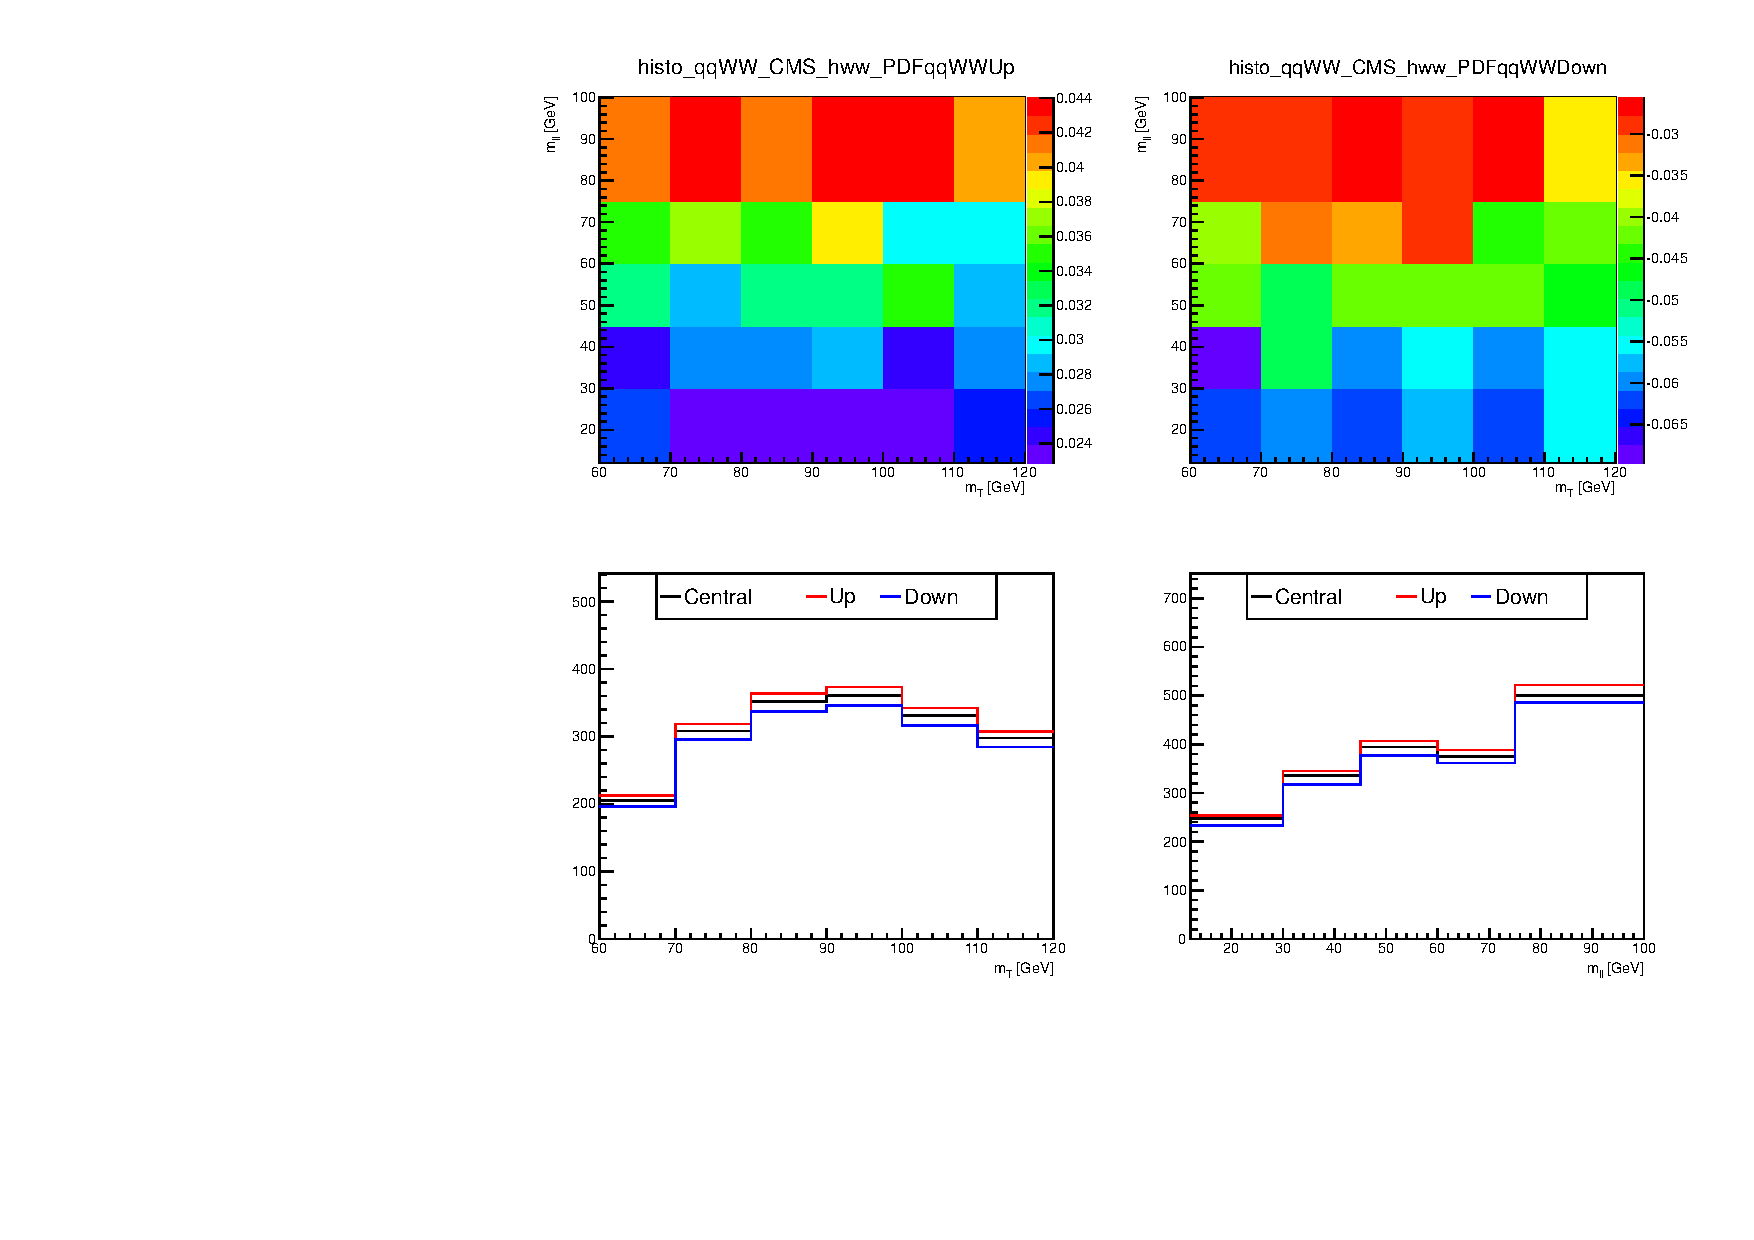
\includegraphics[width=0.8\textwidth]{figures/histo_qqWW_CMS_hww_PDFqqWW_0j_zoom.pdf} 
\end{tabular} 
\caption{ \qqww\ PDF+$\alpha_s$ in 0-jet}
\label{fig:alter_pdfqqww} 
\end{figure} 
%
\begin{figure}[htp] 
\centering 
\begin{tabular}{c} 
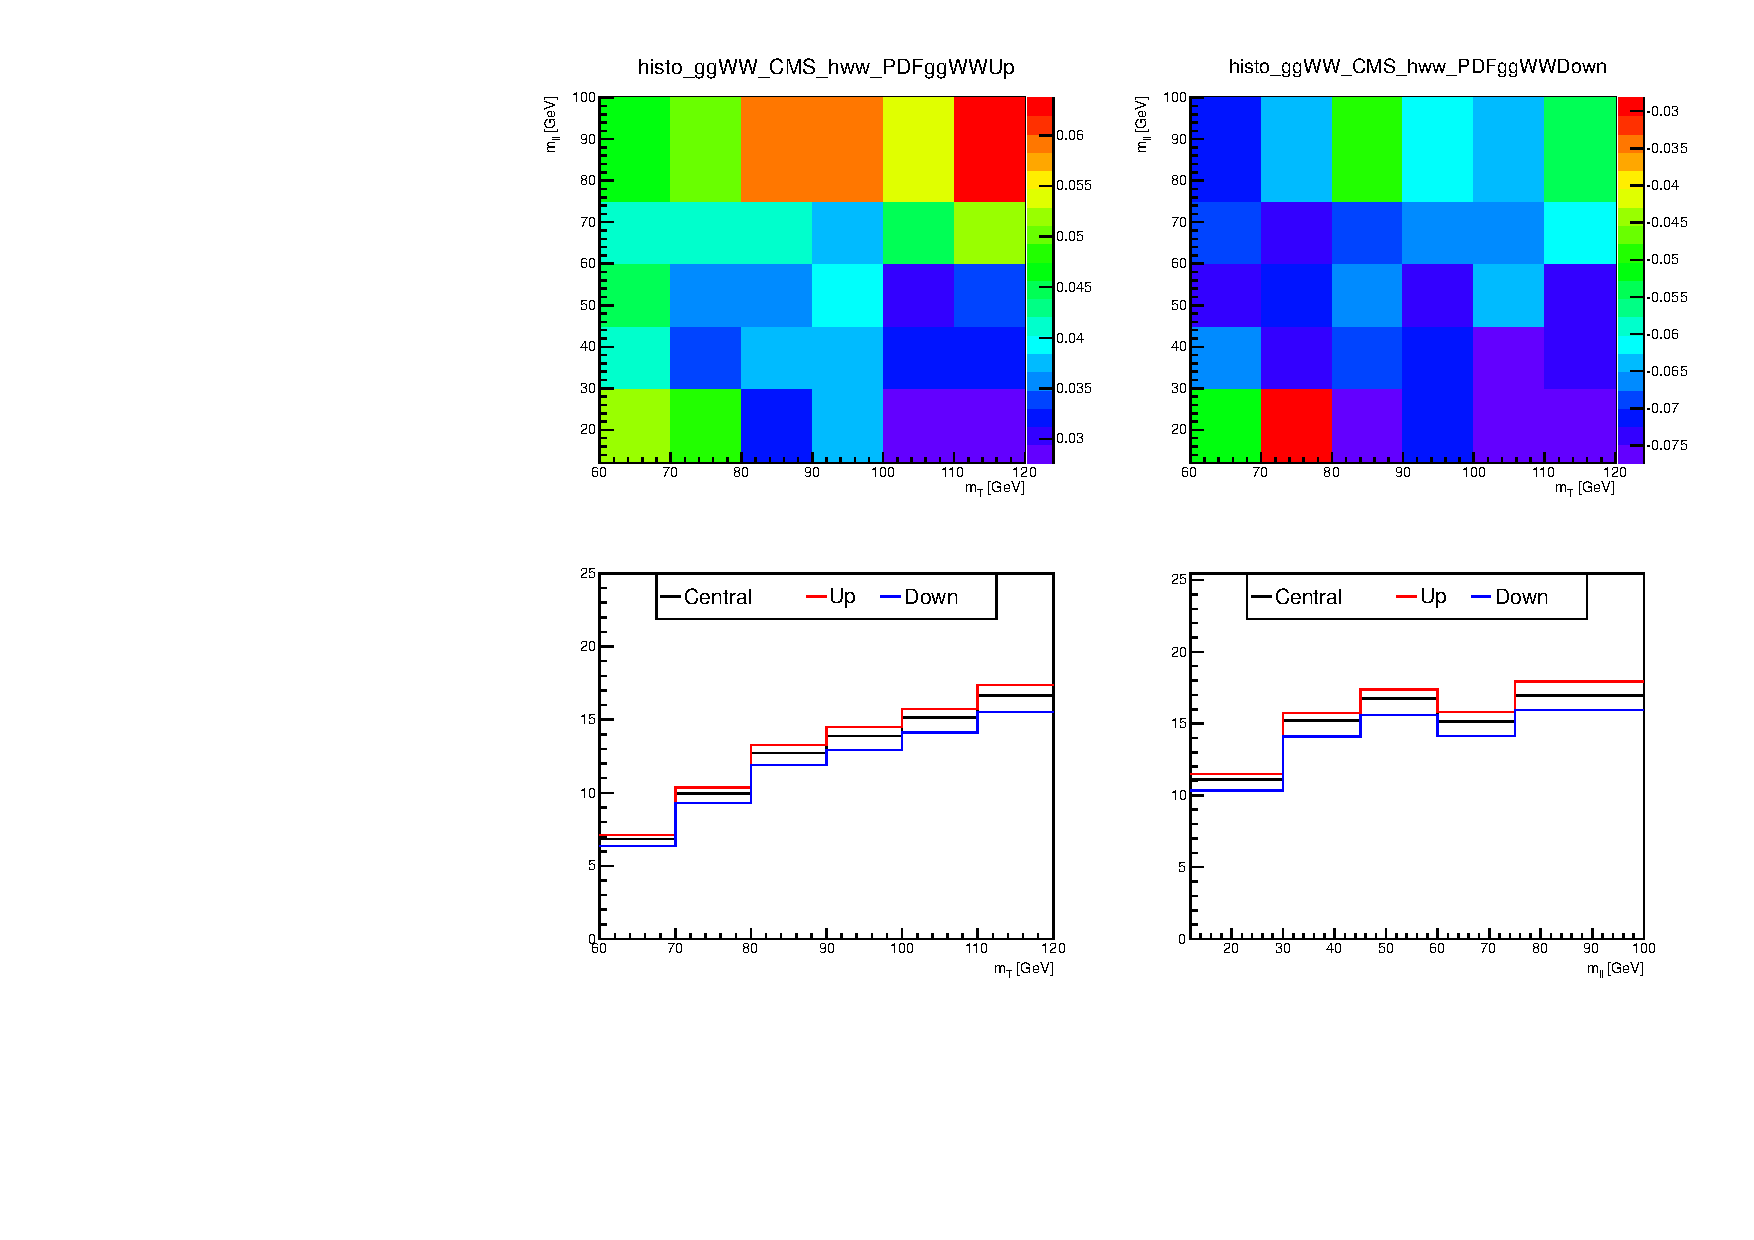
\includegraphics[width=0.8\textwidth]{figures/histo_ggWW_CMS_hww_PDFggWW_0j_zoom.pdf} 
\end{tabular} 
\caption{ \ggww\ PDF+$\alpha_s$ in 0-jet}
\label{fig:alter_pdfggww} 
\end{figure} 

%\subsubsection{QCD Renormalization and factorization scale variation} 
\subsubsection{Missing higher order corrections} 

The cross section of a paricular process is calculated by a pertubation expansion, 
where the first few orders are considered due to complication of calculation 
with higher order terms. In case of SM Higgs production, the cross sections is calculated 
up to NNLO in QCD as shown in tab.~\ref{tab:Higgs_XS_8TeV_order}. Missing next orders 
in the calculation should be accounted for in some way, and this is done by 
varying renormalization scale(\mR) and the factorization scale(\mF) 
by a factor of 2 or 1/2~\cite{}. 

For the \ggH\ process and \qqww\ process for $\mHi>200~\GeV$, 
this effect is expressed in terms of uncertainty to the 
exclusive jet bins and will be discussed in detail in section~\ref{}. 
For other process, the uncertainty due to QCD scale variation ranges from 1 - 4~\%.   

In the shape-based analysis, the effect of \mR\ and \mF\ variation to shape 
is considered for \qqww. The MC@NLO generator is used for matrix element calculation 
with different choice of scales. Up variation corresponds to $\mR=0.5\mu$ and $\mR=2.0\mu$,
and down variation corresponds to $\mR=2.0\mu$ and $\mR=0.5\mu$ where $\mu$ is the nominal 
scale value. Fig.~\ref{fig:alter_qqwwnlo} shows the up and down  
shapes in 2-dimensional template and its projection to \mT\ and \mll\ axes
in the signal region.

Another way of include the effect of missing higher order corrections 
is to compare results calculated in different orders. For \qqww\ and \topbkg\ 
backgrounds we have shape systematics that compares two different simulations. 
For \qqww\ an alternate sample generated by MC@NLO which is calculated up to NLO
is used to define up variation 
and the mirror with repect to the central shape(Madgraph) which is calculated up to LO 
is used as down varition.
Fig.~\ref{fig:alter_qqww} shows the up/down alternate shapes. 
The MC@NLO sample used different parton shower model, Herwig as opposed to 
Pythia used by the default sample, it also accounts for effect of uncertainty 
to modeling of parton shower. 
For \topbkg\ an alternate sample generated by Madgraph which is calculated up to LO
is used to define up variation
and the mirror with repect to the central shape(Powheg) which is calculated up to NLO 
is used as down varition.
Fig.~\ref{fig:alter_qqww} shows the up/down alternate shapes. 

%
\begin{figure}[htp]
\centering
\begin{tabular}{c}
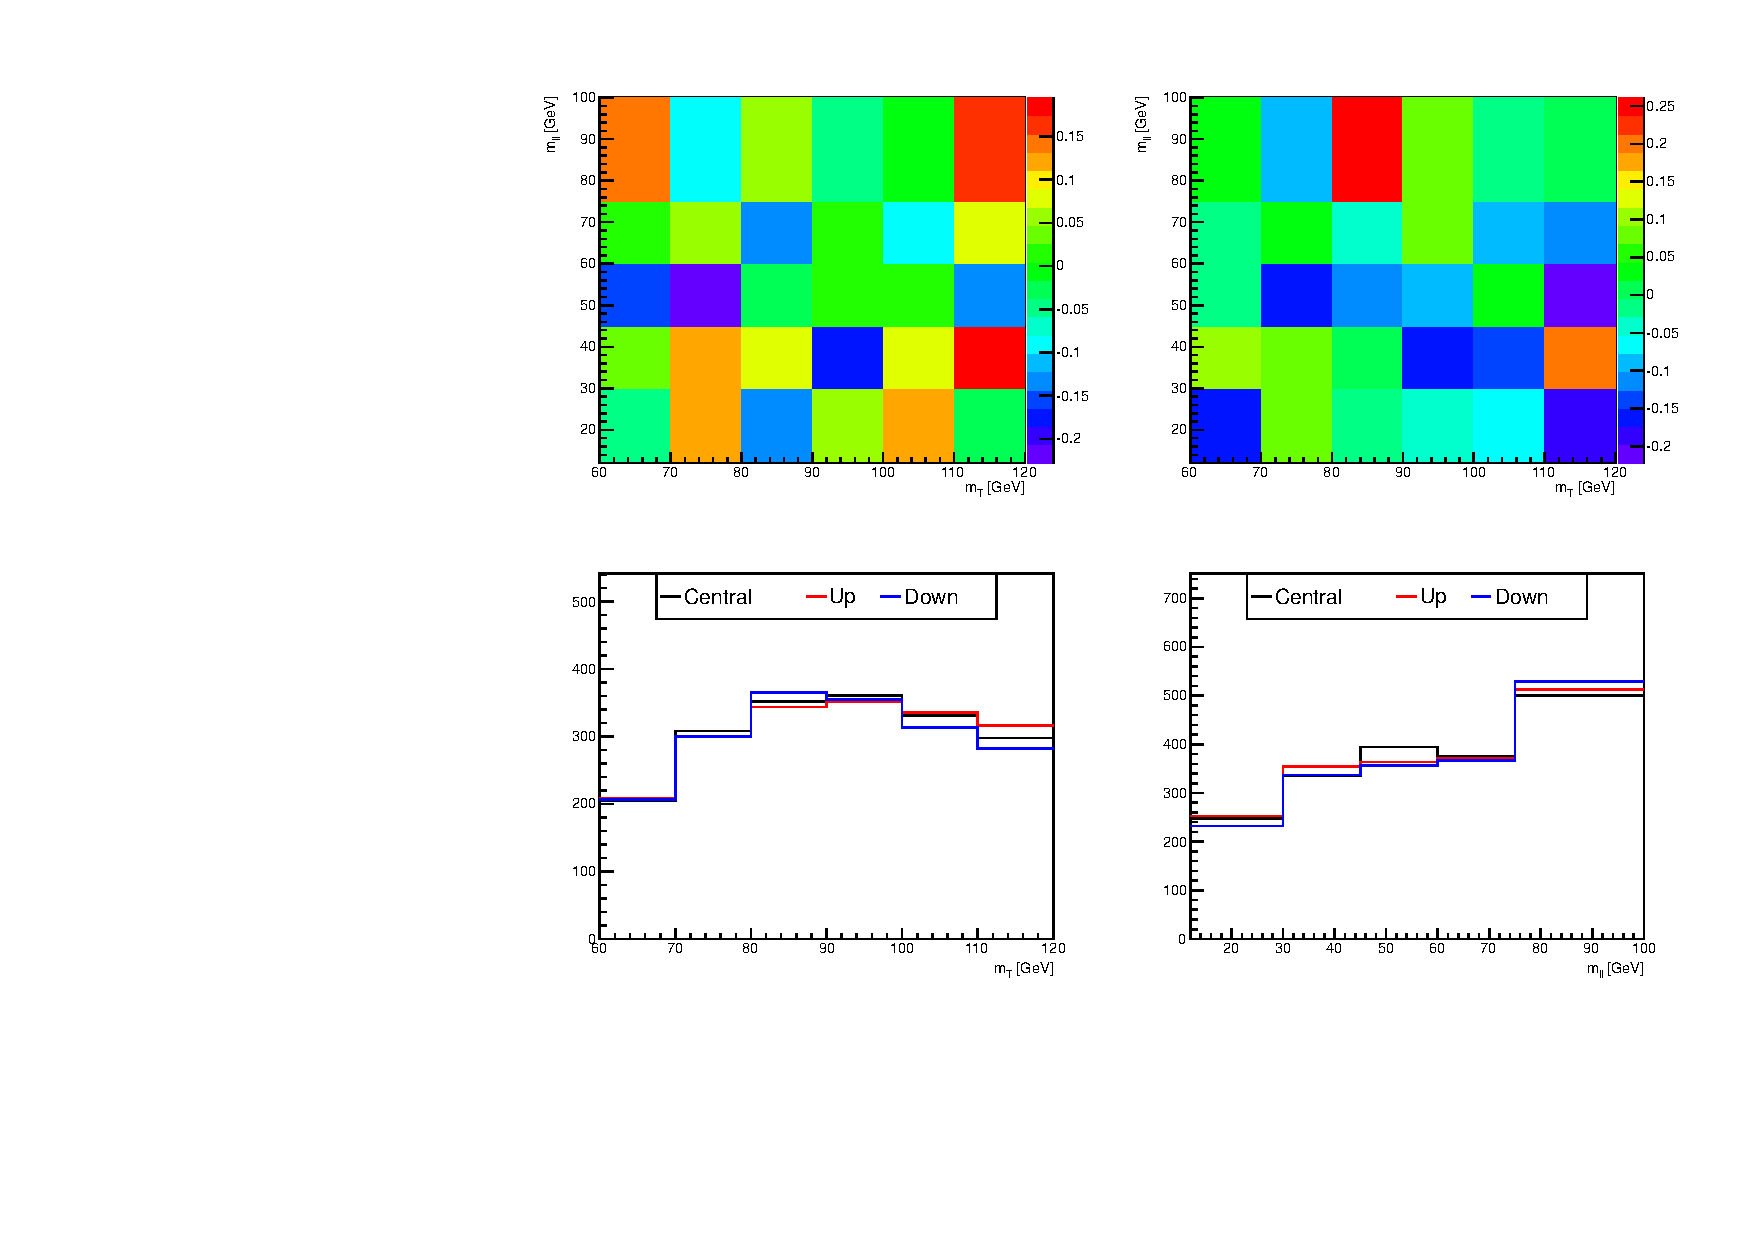
\includegraphics[width=0.8\textwidth]{figures/histo_qqWW_CMS_hww_MVAWWNLOBounding_0j_zoom.pdf}
\end{tabular}
\caption{ \qqww\ QCD scale variation in 0-jet}
\label{fig:alter_qqwwnlo}
\end{figure}
%
\begin{figure}[htp]
\centering
\begin{tabular}{c}
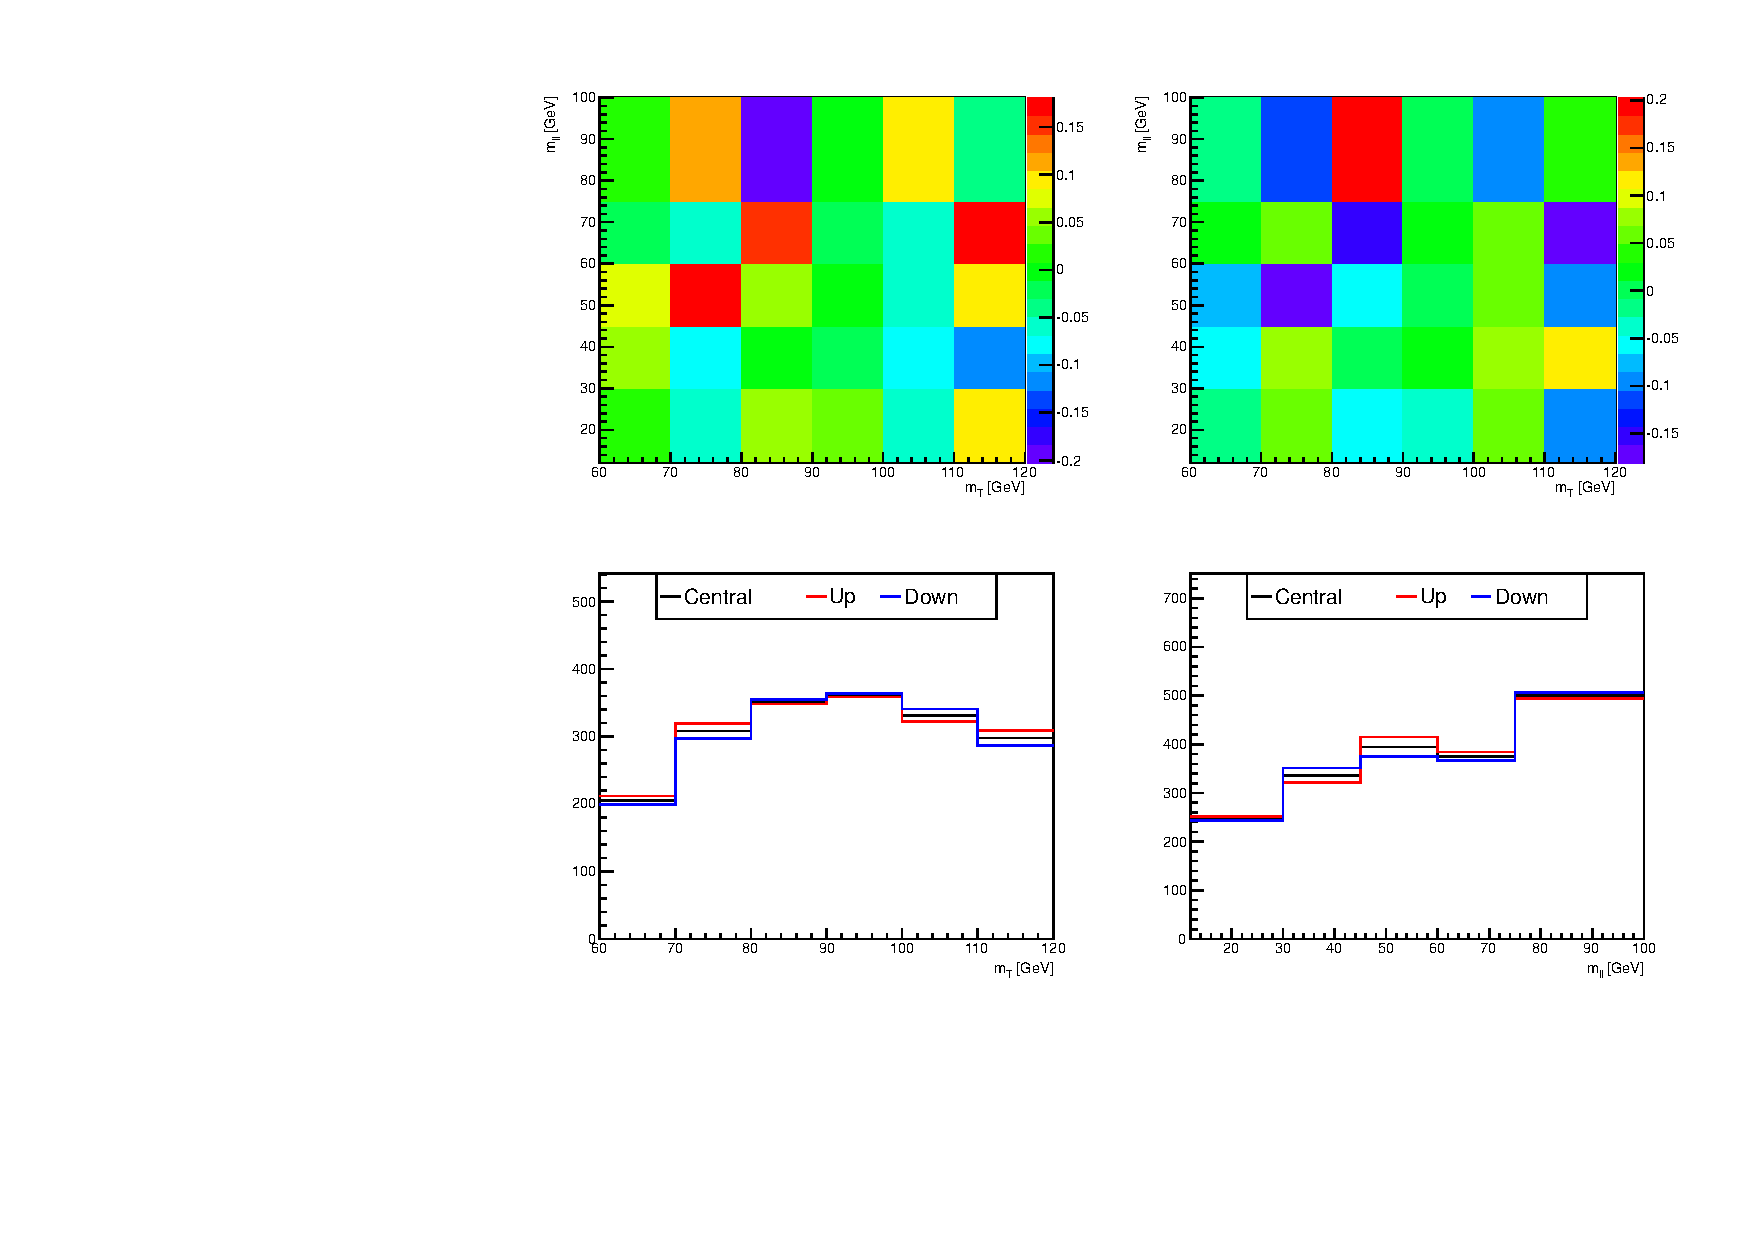
\includegraphics[width=0.8\textwidth]{figures/histo_qqWW_CMS_hww_MVAWWBounding_0j_zoom.pdf}
\end{tabular}
\caption{ \qqww\ Madgraph vs. MC@NLO in 0-jet}
\label{fig:alter_qqww}
\end{figure}
%
\begin{figure}[htp]
\centering
\begin{tabular}{c}
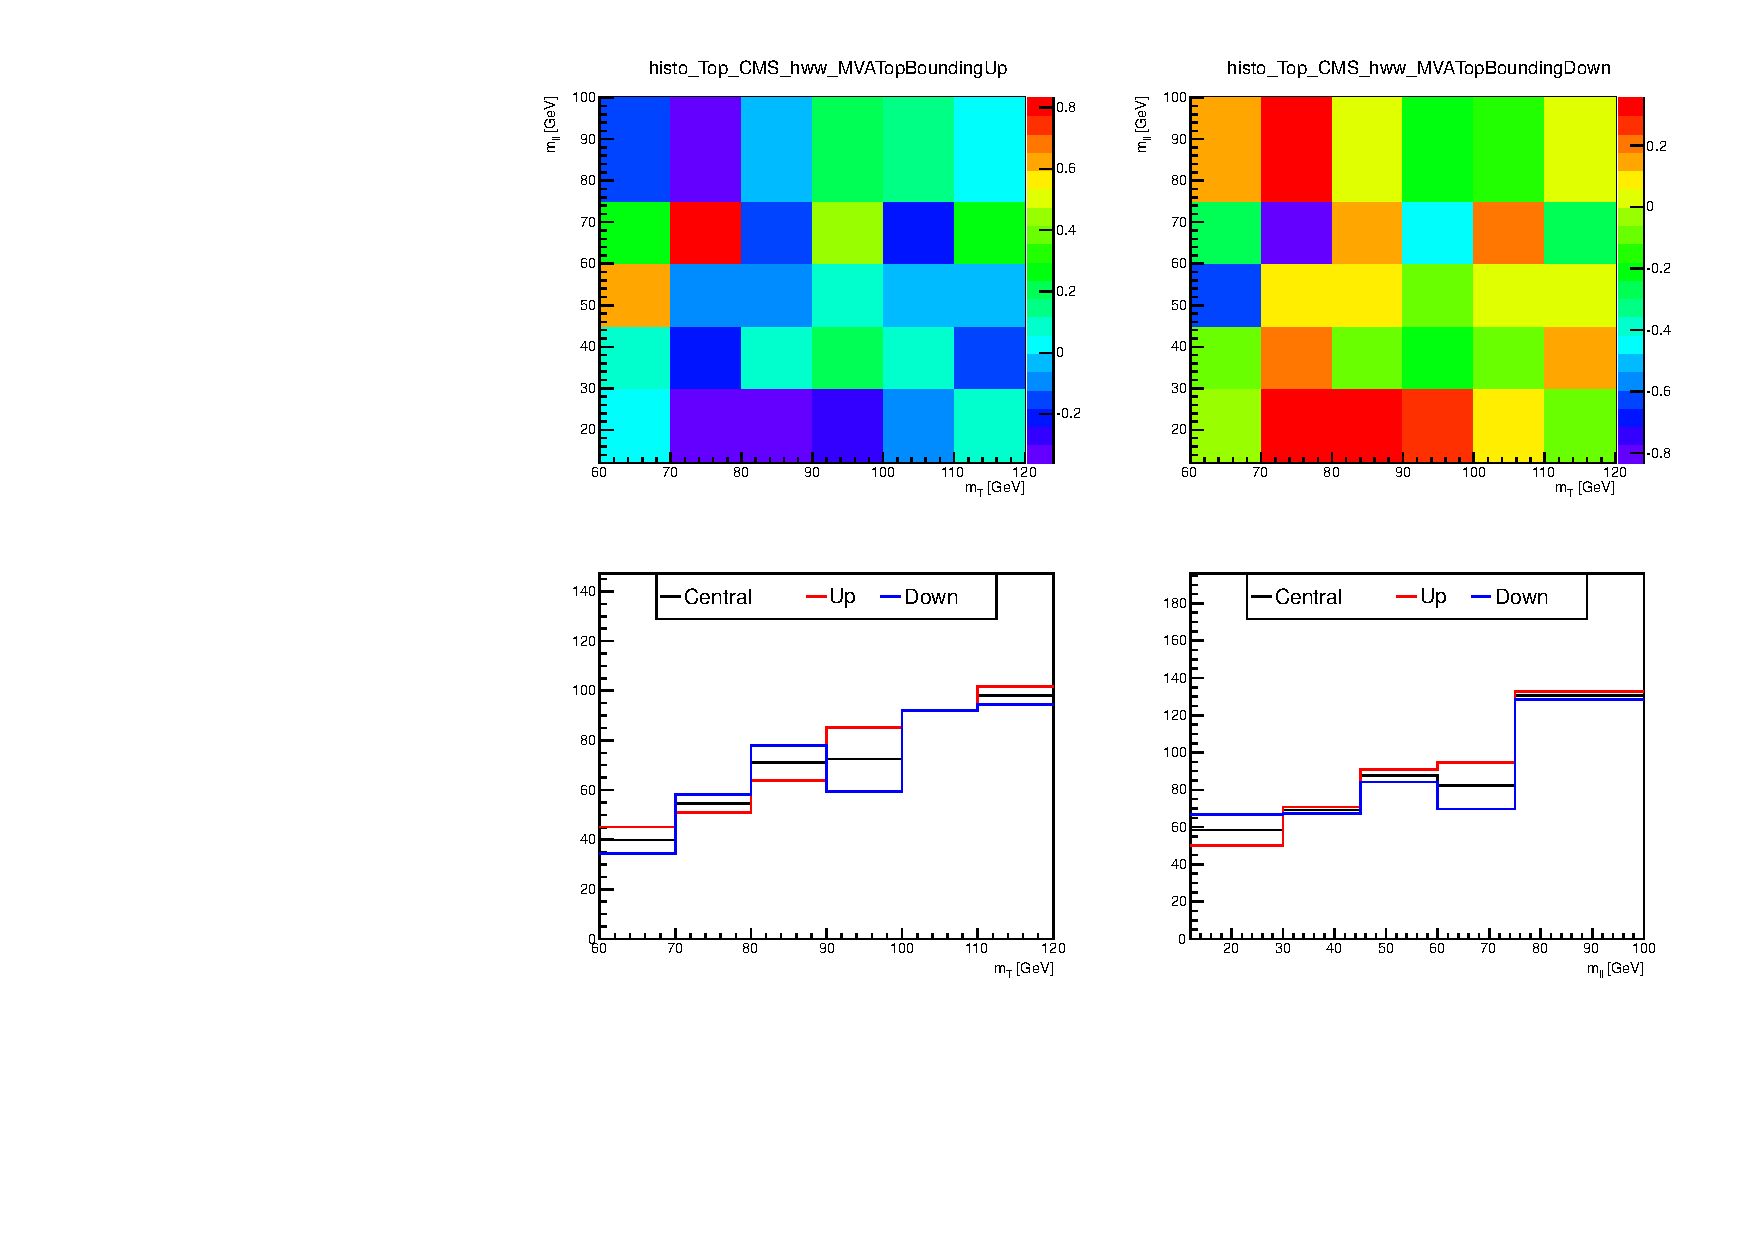
\includegraphics[width=0.8\textwidth]{figures/histo_Top_CMS_hww_MVATopBounding_1j_zoom.pdf}
\end{tabular}
\caption{ \topbkg\ Powheg vs. Madgraph in 1-jet}
\label{fig:alter_top}
\end{figure}

%%%
\subsubsection{Parton shower and underlying events}

The effect of uncertainty in modeling of parton shower(PS) and underlying events(UE) 
is evaluated by comparing different generators using different PS and UE models.
In this analysis, simultions that use Powheg for ME calculation interfaced with Pythia for PS 
that use MC@NLO for ME calculation interfaced with Herwig for PS. 
\textcolor{red}{what about the UE models? How are they different?}
In order to exclude the effect of using different ME calculators, 
the Higgs \pt\ is normalized to the reference distribution~\cite{}.
The tab.~\ref{tab:UEPS} shows the $\kappa$ values of the PS/UE uncertainty 
for a given \mHi. 
%
\begin{table}[htp] 
\begin{center} 
\begin{tabular}{c|ccc} 
\hline 
\mHi\ [\GeV]  & 0-jet & 1-jet & 2-jet \\
\hline \hline 
115 & 0.941 & 1.128 & 1.212 \\   
120 & 0.940 & 1.110 & 1.293 \\   
130 & 0.937 & 1.113 & 1.237 \\   
140 & 0.941 & 1.104 & 1.168 \\   
150 & 0.942 & 1.093 & 1.156 \\   
160 & 0.943 & 1.084 & 1.138 \\   
170 & 0.946 & 1.075 & 1.108 \\   
180 & 0.947 & 1.067 & 1.092 \\   
190 & 0.948 & 1.068 & 1.083 \\   
200 & 0.952 & 1.055 & 1.059 \\   
250 & 0.955 & 1.058 & 0.990 \\   
300 & 0.958 & 1.061 & 0.942 \\   
350 & 0.964 & 1.068 & 0.889 \\   
400 & 0.966 & 1.078 & 0.856 \\   
450 & 0.954 & 1.092 & 0.864 \\   
500 & 0.946 & 1.102 & 0.868 \\   
550 & 0.931 & 1.117 & 0.861 \\   
600 & 0.920 & 1.121 & 0.872 \\   
\hline 
\end{tabular} 
\caption{$\kappa$ values of systematic uncertainty due to modeling of parton showering and underlying events.} 
\label{tab:UEPS} 
\end{center} 
\end{table} 


%%%
\subsubsection{Jet Bin Fractions}

The analysis is optimized by the number of jets and the jets are counted with the requirement that  
its transverse momentum is greater than 30~\GeV. For the processes that the yields in the 
different jet bins are estimated by data-driven methods, there is not related uncertainty 
because the fraction of events in the different jet bins comes from data. On the other hand, 
the processes taken from simulation, for example, \qqH or \qqww\ at $\mHi>200~\GeV$, 
we need to account for this effect.    
The fraction of events that fall into a particular jet bin is affected by the kinematics of events 
and the kinematics of events is affected by missing higher order terms. 
In order to account for this effect, we evaluate the relevant uncertainty by varying 
QCD scales without any additional selection cuts on the signal.

We first get the fraction of jet bins, $f_\textrm{0-jet}$ for $\textrm{0-jet}$, 
$f_\textrm{1-jet}$ for $\textrm{1-jet}$ 
and $f_\textrm{2-jet}$ for $\ge\textrm{2-jet}$ where the fractions are defined as 
\begin{eqnarray} 
f_\textrm{0-jet} 
&=&  
\frac{\sigma_{\ge\textrm{0-jet}} - \sigma_{\ge\textrm{1-jet}}}{\sigma_{\ge\textrm{0-jet}}} \\
f_\textrm{1-jet} 
&=&  
\frac{\sigma_{\ge\textrm{1-jet}} - \sigma_{\ge\textrm{2-jet}}}{\sigma_{\ge\textrm{0-jet}}} \\
f_\textrm{2-jet} 
&=&  
\frac{\sigma_{\ge\textrm{2-jet}}}{\sigma_{\ge\textrm{0-jet}}} 
\end{eqnarray}  
The systematic uncertainties on the inclusive cross sections, 
$\sigma_{\ge\textrm{0-jet}}$, $\sigma_{\ge\textrm{1-jet}}$ and $\sigma_{\ge\textrm{2-jet}}$ are 
manifested by $\kappa_{\ge\textrm{0-jet}}$, $\kappa_{\ge\textrm{1-jet}}$ and $\kappa_{\ge\textrm{2-jet}}$, repectively.
The central values of the inclusive cross sections are calculated 
using MSTW2008 NLO PDF at the QCD scales, $\mR=\mF=\mHi/2$.
The uncertainty on the $\sigma_{\ge\textrm{0-jet}}$, $\kappa_{\ge\textrm{0-jet}}$, is taken from the 
CERN Yellow Report~\cite{Dittmaier:1318996}, and the uncertainties 
on $\sigma_{\ge\textrm{1-jet}}$ and $\sigma_{\ge\textrm{2-jet}}$, $\kappa_{\ge\textrm{1-jet}}$ and $\kappa_{\ge\textrm{2-jet}}$, are 
calculated by the following QCD scale variations using MCFM~\cite{}: 
\begin{itemize}
\item $\mF = \mHi $, $\mR = \mHi$,
\item $\mF = \mHi / 4$, $\mR = \mHi / 4$,
\item $\mF = \mHi $, $\mR = \mHi / 2$,
\item $\mF = \mHi / 2$, $\mR= \mHi $,
\end{itemize}
\textcolor{red}{Is this a recommendation by Higgs Cross Section WG?} 
The largest positive($\Delta_{+}$) and negative($\Delta_{-}$) uncertainties 
to $\sigma_{\ge\textrm{1-jet}}$ and $\sigma_{\ge\textrm{2-jet}}$ are taken 
and they are symmetrized to be expressed in terme of $\kappa$. 
The symmetrization is done by 
\begin{eqnarray} 
  \kappa_{\mathrm{symmetrized}} = \sqrt{e^{\Delta_{+}} \times e^{\Delta_{-}}} ,
\end{eqnarray} 
where the $\kappa_{\mathrm{symmetrized}}$ is the resultant $\kappa$
for the asymmetric uncertainties, $\Delta_{+}$ and $\Delta_{-}$.
Using the values in tab~\ref{tab:jetbinincl}, we can convert the inclusive jet bin 
uncertainties to exclusive jet bin uncertainties by the formulae shown in tab.~\ref{tab:jetbinexcl}~\cite{}.
\begin{table}[!htbp]
\begin{center}
\begin{tabular}{c|ccc}

\hline
Nuisance Parameter & $\kappa$'s for 0-jet bin   & $\kappa$'s for 1-jet bin  & $\kappa$'s for 2-jet bin                       \\
\hline \hline
$\theta_{\textrm{from } \ge \textrm{0-jet}}$  & $ (\kappa_{\geq 0})^{\frac{1}{f_\textrm{0-jet}}}$    & $1.0$ & $1.0$                                            \\
$\theta_{\textrm{from } \ge \textrm{1-jet}}$  & $(\kappa_{\geq 1})^{- \frac{f_\textrm{1-jet}+f_\textrm{2-jet}}{f_\textrm{0-jet}}}$ & $(\kappa_{\geq 1})^{\frac{f_\textrm{1-jet}+f_\textrm{2-jet}}{f_\textrm{1-jet}}}$  & $1.0$                                            \\
$\theta_{\textrm{from } \ge \textrm{2-jet}}$  & $1.0$ & $(\kappa_{\geq 2})^{- \frac{f_\textrm{2-jet}}{f_\textrm{1-jet}}} $     & $\kappa_{\geq 2}$ \\
\hline

\end{tabular}
\caption{Table of formulae expressing the $\kappa$ values for the systematic uncertainties on the
jet bin fractions due to the missing higher order corrections on 
$\sigma_{\ge\textrm{0-jet}}$, $\sigma_{\ge\textrm{1-jet}}$ and $\sigma_{\ge\textrm{2-jet}}$,
in terms of the $\kappa$ values for these cross sections, 
$\kappa_{\ge\textrm{0-jet}}$, $\kappa_{\ge\textrm{1-jet}}$ and $\kappa_{\ge\textrm{2-jet}}$, respectively, 
and the jet bin fractions, 
$f_{\textrm{0-jet}}$, $f_{\textrm{1-jet}}$ and $f_{\textrm{2-jet}}$.
}
\label{tab:jetbinformula}
\end{center}
\end{table}

For \ggH process, the numerical values of $\kappa_{\ge\textrm{0-jet}}$, $\kappa_{\ge\textrm{1-jet}}$ 
and $\kappa_{\ge\textrm{2-jet}}$ are summurized in tab.~\ref{tab:jetbinincl}.
%
\begin{table}[!htbp]
\begin{center}
\begin{tabular}{c|ccc}
\hline
\mHi[\GeV]    &     $\kappa_{\ge\textrm{0-jet}}$        &   $\kappa_{\ge\textrm{1-jet}}$        &     $\kappa_{\ge\textrm{2-jet}}$       \\
\hline\hline
 115 & $ 1.106$  & $ 1.226$  & $ 1.149$  \\
 120 & $ 1.104$  & $ 1.224$  & $ 1.120$  \\
 130 & $ 1.100$  & $ 1.230$  & $ 1.117$  \\
 140 & $ 1.096$  & $ 1.220$  & $ 1.129$  \\
 150 & $ 1.095$  & $ 1.220$  & $ 1.124$  \\
 160 & $ 1.095$  & $ 1.221$  & $ 1.199$  \\
 170 & $ 1.090$  & $ 1.222$  & $ 1.175$  \\
 180 & $ 1.089$  & $ 1.218$  & $ 1.171$  \\
 190 & $ 1.087$  & $ 1.217$  & $ 1.171$  \\
 200 & $ 1.087$  & $ 1.213$  & $ 1.197$  \\
 250 & $ 1.083$  & $ 1.208$  & $ 1.230$  \\
 300 & $ 1.082$  & $ 1.208$  & $ 1.205$  \\
 350 & $ 1.090$  & $ 1.207$  & $ 1.209$  \\
 400 & $ 1.075$  & $ 1.195$  & $ 1.195$  \\
 450 & $ 1.078$  & $ 1.194$  & $ 1.196$  \\
 500 & $ 1.087$  & $ 1.188$  & $ 1.174$  \\
 550 & $ 1.089$  & $ 1.191$  & $ 1.194$  \\
 600 & $ 1.090$  & $ 1.187$  & $ 1.192$  \\

\hline
\end{tabular}
\caption{ $\kappa$ values for the systematic uncertainties due to missing higher order corrections
for the inclusive \ggH\ production cross section, 
$\sigma_{\ge\textrm{0-jet}}$, $\sigma_{\ge\textrm{1-jet}}$ and $\sigma_{\ge\textrm{2-jet}}$. 
The corresponding $\kappa$s are $\kappa_{\ge\textrm{0-jet}}$, $\kappa_{\ge\textrm{1-jet}}$ 
and $\kappa_{\ge\textrm{2-jet}}$, respectively. 
}
\label{tab:jetbinincl}
\end{center}
\end{table}
Combining information in tab.~\ref{tab:jetbinincl} and tab.~\ref{tab:jetbinformula} 
we obtain the final $\kappa$'s for \ggH\ process as shown in tab.~\ref{tab:jetbinexcl}.
%
\begin{table}[!htbp]
\begin{center}
\begin{tabular}{c|cc|cc|c}

\hline
\multirow{2}{*}{\mHi [\GeV]} 
               & \multicolumn{2}{c|}{0-jet bin}  & \multicolumn{2}{c|}{1-jet bin}  & 2-jet bin \\ 
               & $\kappa_{\mathrm{from } \ge \textrm{0-jet}}$ & $\kappa_{\mathrm{from } \ge \textrm{1-jet}}$ 
               & $\kappa_{\mathrm{from } \ge \textrm{1-jet}}$ & $\kappa_{\mathrm{from } \ge \textrm{2-jet}}$  
               & $\kappa_{\mathrm{from } \ge \textrm{2-jet}}$   \\
\hline \hline
 115 & $ 1.16$  & $ 0.92$  & $ 1.28$  & $ 0.97$  & $ 1.15$  \\
 120 & $ 1.16$  & $ 0.92$  & $ 1.28$  & $ 0.97$  & $ 1.12$  \\
 130 & $ 1.15$  & $ 0.91$  & $ 1.29$  & $ 0.98$  & $ 1.12$  \\
 140 & $ 1.15$  & $ 0.91$  & $ 1.28$  & $ 0.97$  & $ 1.13$  \\
 150 & $ 1.15$  & $ 0.90$  & $ 1.28$  & $ 0.97$  & $ 1.12$  \\
 160 & $ 1.15$  & $ 0.90$  & $ 1.28$  & $ 0.96$  & $ 1.20$  \\
 170 & $ 1.15$  & $ 0.89$  & $ 1.28$  & $ 0.96$  & $ 1.18$  \\
 180 & $ 1.15$  & $ 0.89$  & $ 1.28$  & $ 0.96$  & $ 1.17$  \\
 190 & $ 1.15$  & $ 0.88$  & $ 1.28$  & $ 0.96$  & $ 1.17$  \\
 200 & $ 1.15$  & $ 0.88$  & $ 1.27$  & $ 0.96$  & $ 1.20$  \\
 250 & $ 1.16$  & $ 0.86$  & $ 1.27$  & $ 0.96$  & $ 1.17$  \\
 300 & $ 1.17$  & $ 0.84$  & $ 1.27$  & $ 0.95$  & $ 1.20$  \\
 350 & $ 1.20$  & $ 0.83$  & $ 1.27$  & $ 0.95$  & $ 1.21$  \\
 400 & $ 1.17$  & $ 0.82$  & $ 1.26$  & $ 0.95$  & $ 1.20$  \\
 450 & $ 1.19$  & $ 0.81$  & $ 1.26$  & $ 0.95$  & $ 1.20$  \\
 500 & $ 1.22$  & $ 0.80$  & $ 1.25$  & $ 0.95$  & $ 1.17$  \\
 550 & $ 1.24$  & $ 0.78$  & $ 1.26$  & $ 0.95$  & $ 1.19$  \\
 600 & $ 1.25$  & $ 0.78$  & $ 1.26$  & $ 0.94$  & $ 1.19$  \\

\hline

\end{tabular}
\caption{ Table of $\kappa$ values for the systematic uncertainties for the jet bin 
fractions due to missing higher order corrections for the total inclusive Higgs
cross section, the inclusive Higgs+1jet cross section, and the inclusive Higgs+2jet
cross section. }
\label{tab:jetbinexcl}
\end{center}
\end{table}

For \qqww\ process, the inclusive cross sections, $\sigma_{\ge\textrm{0-jet}}$,
$\sigma_{\ge\textrm{1-jet}}$ and $\sigma_{\ge\textrm{2-jet}}$ are evaluated using MC@NLO~\cite{} 
and the corresponding uncertainties are estimated by combination of  
QCD scale variation and comparison with ALPGEN~\cite{}. 
The uncertainties to the above inclusive cross sections are 3~\%,  6~\% and 42~\% for  
$\sigma_{\ge\textrm{0-jet}}$, $\sigma_{\ge\textrm{1-jet}}$ and $\sigma_{\ge\textrm{2-jet}}$,
respectively.  
The jet bin fractions calculated using the inclusive cross sections are 
$f_{\textrm{0-jet}}=0.70$, $f_{\textrm{1-jet}}=0.22$ and $f_{\textrm{2-jet}}=0.08$.
Inserting these numbers into the formulae in tab~\ref{tab:jetbinformula}, 
we obtain the $\kappa$'s of the jet bin fraction uncertainties for \qqww\ process
as shown in tab.~\ref{tab:jetbinexcl_ww}. 
%
\begin{table}[!htbp]
\begin{center}
\begin{tabular}{cc|cc|c}
\hline
\multicolumn{2}{c|}{0-jet bin}  & \multicolumn{2}{c|}{1-jet bin}  & 2-jet bin \\
$\kappa_{\mathrm{from } \ge \textrm{0-jet}}$ & $\kappa_{\mathrm{from } \ge \textrm{1-jet}}$
& $\kappa_{\mathrm{from } \ge \textrm{1-jet}}$ & $\kappa_{\mathrm{from } \ge \textrm{2-jet}}$
& $\kappa_{\mathrm{from } \ge \textrm{2-jet}}$   \\
\hline \hline
$1.042$  & $ 0.978$  & $ 1.076$  & $ 0.914$  & $ 1.42$  \\
\hline
\end{tabular}
\caption{ Table of $\kappa$ values for the systematic uncertainties for the jet bin
fractions due to missing higher order corrections for the total inclusive \qqww\
cross section, the inclusive \qqww+1jet cross section, and the inclusive \qqww+2jet
cross section. }
\label{tab:jetbinexcl_ww}
\end{center}
\end{table}



%%%%%%%%%%%%%%%%%%%%%%%%%%%%%%%%%%%
\section{Instrumental Systematic Uncertainties} 
\begin{itemize} 
\item Luminosity : for 8 TeV which luminosity uncertainty to quote? %4.4\% of 2.6\%? 
      How is the uncertainty estimated?
\item PU : ~1\% so neglected    
\item Lepton momentum scale and resolution (shape for 2D) 
      How is the uncertainty estimated?
\item Lepton efficiency (shape for 2D)    
      How is the uncertainty estimated?
\item MET resolution (shape for 2D)    
      How is the uncertainty estimated?
\item Jet energy scale (shape for 2D)     
      How is the uncertainty estimated? for shape $\pm5\%$ for jet bin migration 
\item  MC statistics shape uncertainty : mention bin-by-bin treatment gives consistent result  
\end{itemize} 


%%%
\subsubsection{Luminosity}

The luminosity at CMS is measured by Hadronic Forward calorimeter(HF)
and silicon pixel detector. Thanks to small dependence on experimental 
conditions such as pileup, the counting of the pixel clusters is chosen 
for the precision luminosity measurement~\cite{CMS-PAS-LUM-13-001}. 
The measured luminosity is calibrated by Van Der Meer Scans at the ISR~\cite{CMS-PAS-LUM-13-001}.
The dominant source of uncertainty is the choice of fit function 
to model bunch shapes.  

The total estimated uncertainties are 2.6~\%~\cite{CMS-PAS-LUM-13-001} at 8~\TeV\ 
and 2.2~\% at 7~\TeV~\cite{}.  

%%%
\subsubsection{Lepton momentum scale and resolution}

The lepton momentum scale and resolution can affect selection efficiency 
fot the cuts applied on lepton momentum or variables constructed from 
lepton momenta. The size of uncertianties of both sources is estimated 
by comparing Z invariant mass shape between simulation and data in \SF\ 
final state. The momentum scale is responsible for the location of the 
invariant mass peak, and the momentum resolution is reposible for the width 
of the distribution. 

The measured uncertainties are 1.5~\%(3~\%) for electrons in barrel(endcap)  
and 1.0~\%(1.7~\%) for muons in barrel(endcap). For the cut-based analysis
we use the average of bareel and endcap, 2~\% for electron and 1.5~\% for muon. 
For the shape-based analysis, new \mT\ and \mll\ are calculated using the 
lepton momenta scaled by the measured resolutions.
The up shape is made by adding the smeared momentum resolution to both leptons
and the down shape is made by subtracting the smeared momentum resolution to both leptons.
Fig.~\ref{fig:alter_lepres} shows the corresponding up/down alternate shapes. 
%
\begin{figure}[htp]
\centering
\begin{tabular}{c}
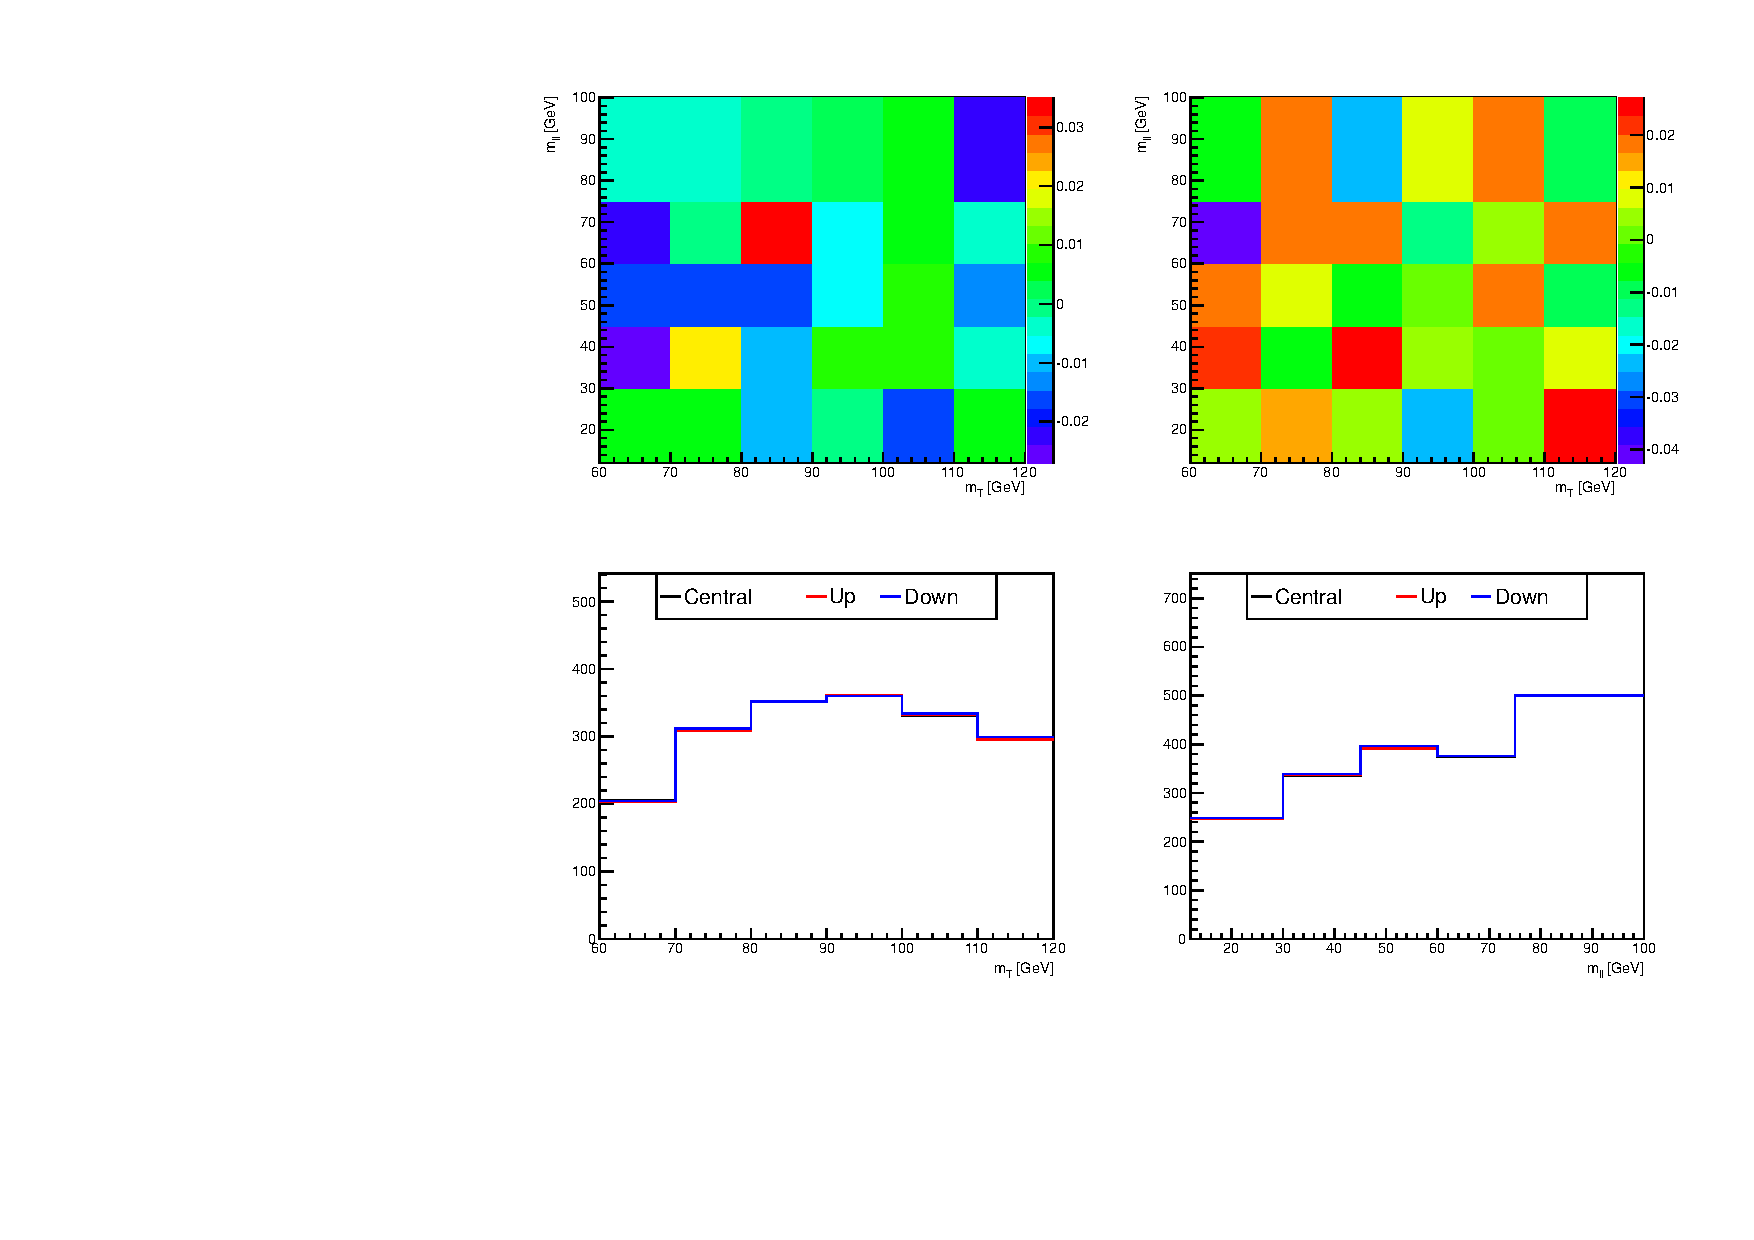
\includegraphics[width=0.8\textwidth]{figures/histo_qqWW_CMS_hww_MVALepResBounding_0j_zoom.pdf}
\end{tabular}
\caption{Alternate shapes for lepton momentum scale and resolution.}
\label{fig:alter_lepres}
\end{figure}


%%%
\subsubsection{Lepton efficiency} 

The lepton selection and trigger efficiencies are measured by Tag-and-Probe method
as described in chapter~\ref{ch:efficiency_measurement}. The uncertainty comes from 
the determination of backgrounds and the modeling of the signal 
and background in the likelihood fit. Additional uncertainty which is 
prominent in the low \pt\ region in the electron case 
comes from the possible bias by use of N-1 technique. 
This is described in section~\ref{sec:electroneff} as well as the corresponding 
unceratinties in tab.~\ref{tab:eff_electron_nmsyst}.

The estimated uncertainties are 3~\% for muons and 4~\% for electrons 
which are used by the cut-based analysis. 
For the shape-based analysis, alternate shapes are constructed by
scaling up/down the event weights using the systematics sources
as a function of lepton \pt\ and \Eta.
Fig.~\ref{fig:alter_lepeff} shows the corresponding up/down alternate shapes. 

%
\begin{figure}[htp]
\centering
\begin{tabular}{c}
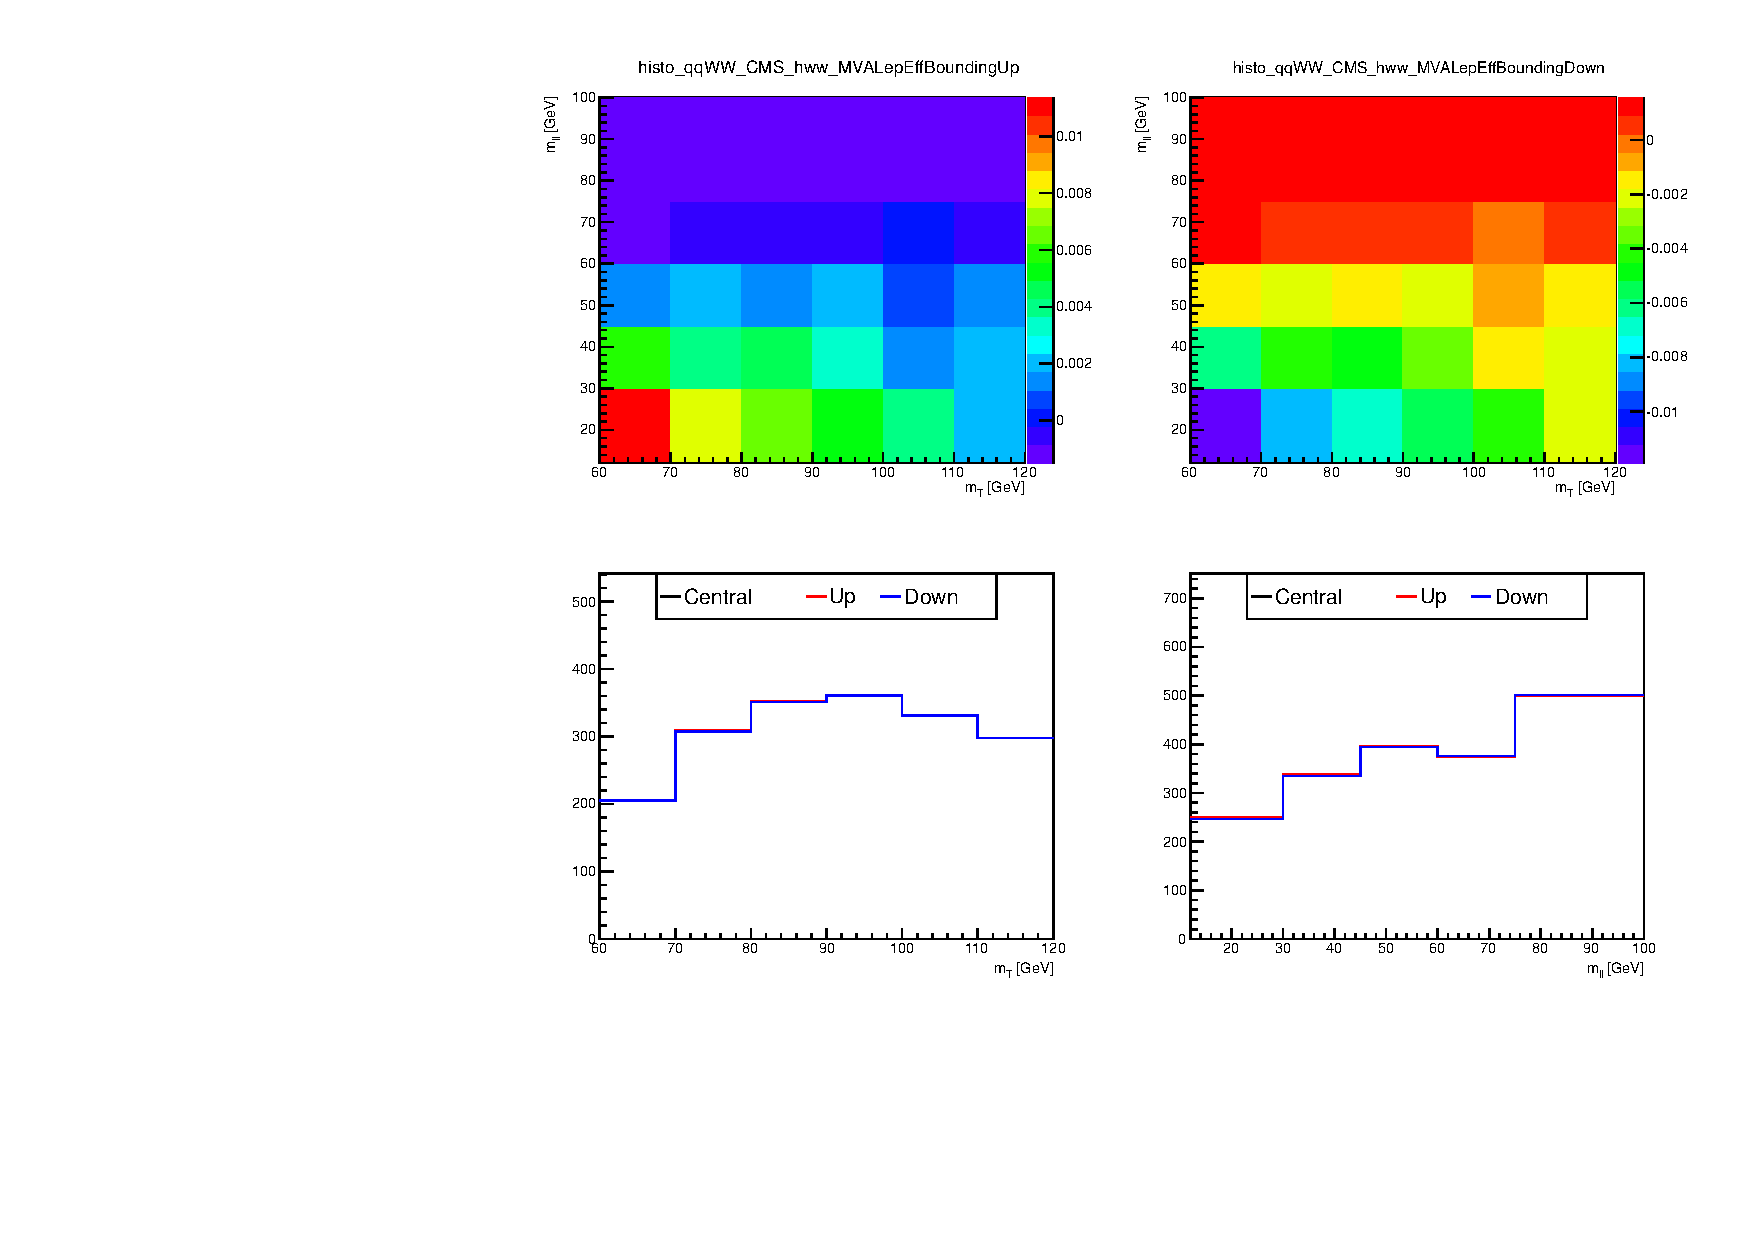
\includegraphics[width=0.8\textwidth]{figures/histo_qqWW_CMS_hww_MVALepEffBounding_0j_zoom.pdf}
\end{tabular}
\caption{Alternate shapes for lepton efficiency. \textcolor{red}{looks too small at low \mT\ and \mll.}}
\label{fig:alter_lepeff}
\end{figure}


%%%
\subsubsection{MET resolution} 

The mis-modeling of \met\ by simulation can introduce systematic uncertainty 
as we select events that pass \met\ selections. The uncertainty is measured 
by comparing data and simulation using \dyll\ events. To account for the 
difference between data and simulation, additional Gaussian smearing for 
the individual x and y compoments of \met\ are needed. 
For PF \met, the size of Gaussian smearing is 3.2 and 3.6~\GeV %and 4.3 
for 0-jet and 1-jet categories, respectively.  
For \trkmet, the size of Gaussian smearing is 1.0 and 4.5~\GeV %and 6.0 
for 0-jet and 1-jet categories, respectively.  

For the cut-based analysis, the resultant effect of smearing is around 2~\%. 
For the shape-based analysis, the up/down alternate shapes are constructed 
by new \mT\ calculated using the smeared x and y components of \met.
Fig.~\ref{fig:alter_lepeff} shows the corresponding up/down alternate shapes. 

%
\begin{figure}[htp]
\centering
\begin{tabular}{c}
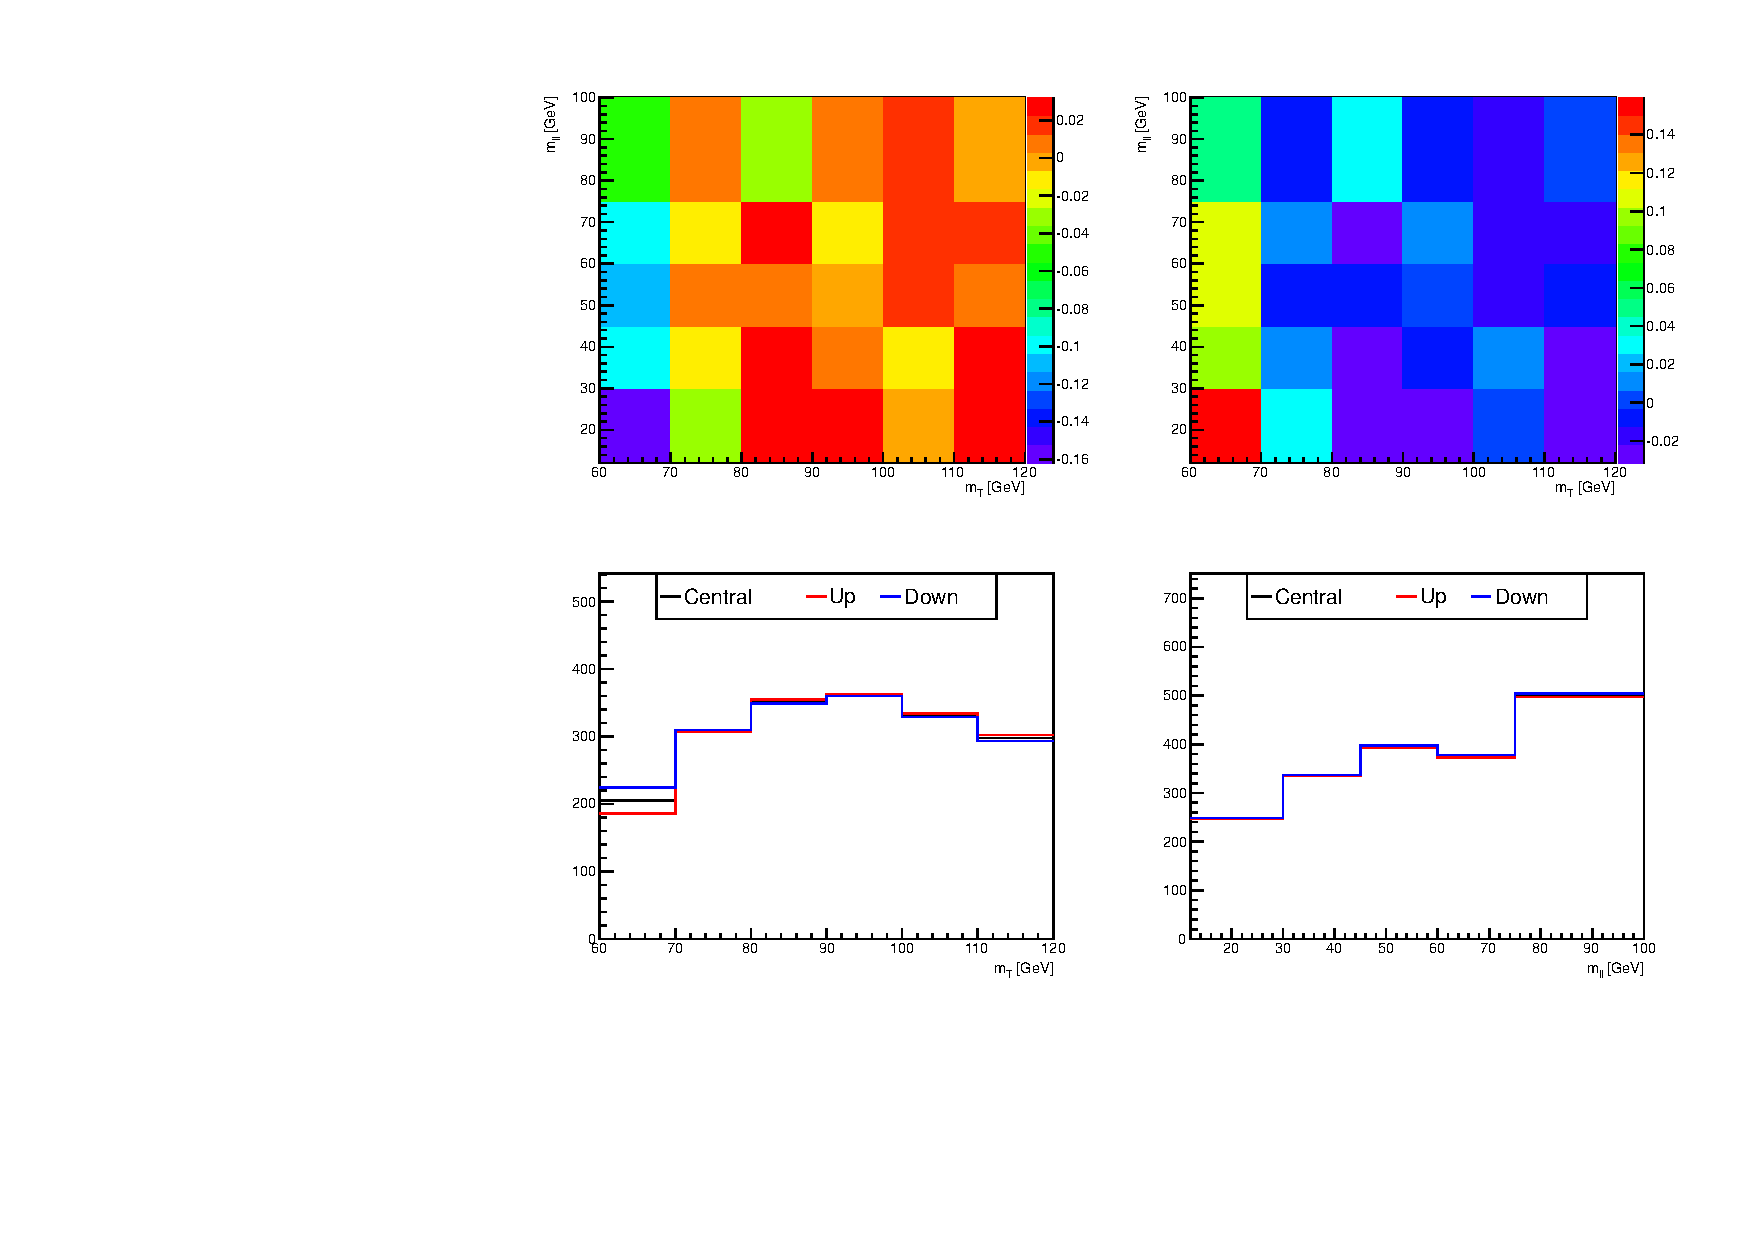
\includegraphics[width=0.8\textwidth]{figures/histo_qqWW_CMS_hww_MVAMETResBounding_0j_zoom.pdf}
\end{tabular}
\caption{Alternate shapes for \met\ resolution.}
\label{fig:alter_metres}
\end{figure}

%%%
\subsubsection{Jet energy scale} 

This analysis is optimized in jet bins and the jet selection is done by 
requiring \pt\ to be greater than 30~\GeV. Thus, uncertainty on the 
energy of jets can lead to biased results. From the studies on the PF jet 
energy resolution are done in \cite{Chatrchyan:2011ds}, the jet energy 
resolution ranges from 3~\% to 5~\% as \Eta\ of jets increase. We take 
5 \% for whole \Eta\ range as a conservative choice.   

For the cut-based analysis, resultant effect of 5~\% of jet energy resolution 
is around 2~\%. 
For the shape-based analysis, the up/down alternate shapes are constructed
by scaling jet transverse momentum by $\pm 5$~\%.
Fig.~\ref{fig:alter_jes} shows the corresponding up/down alternate shapes. 


%FIXME :  I am here

%
\begin{figure}[htp]
\centering
\begin{tabular}{c}
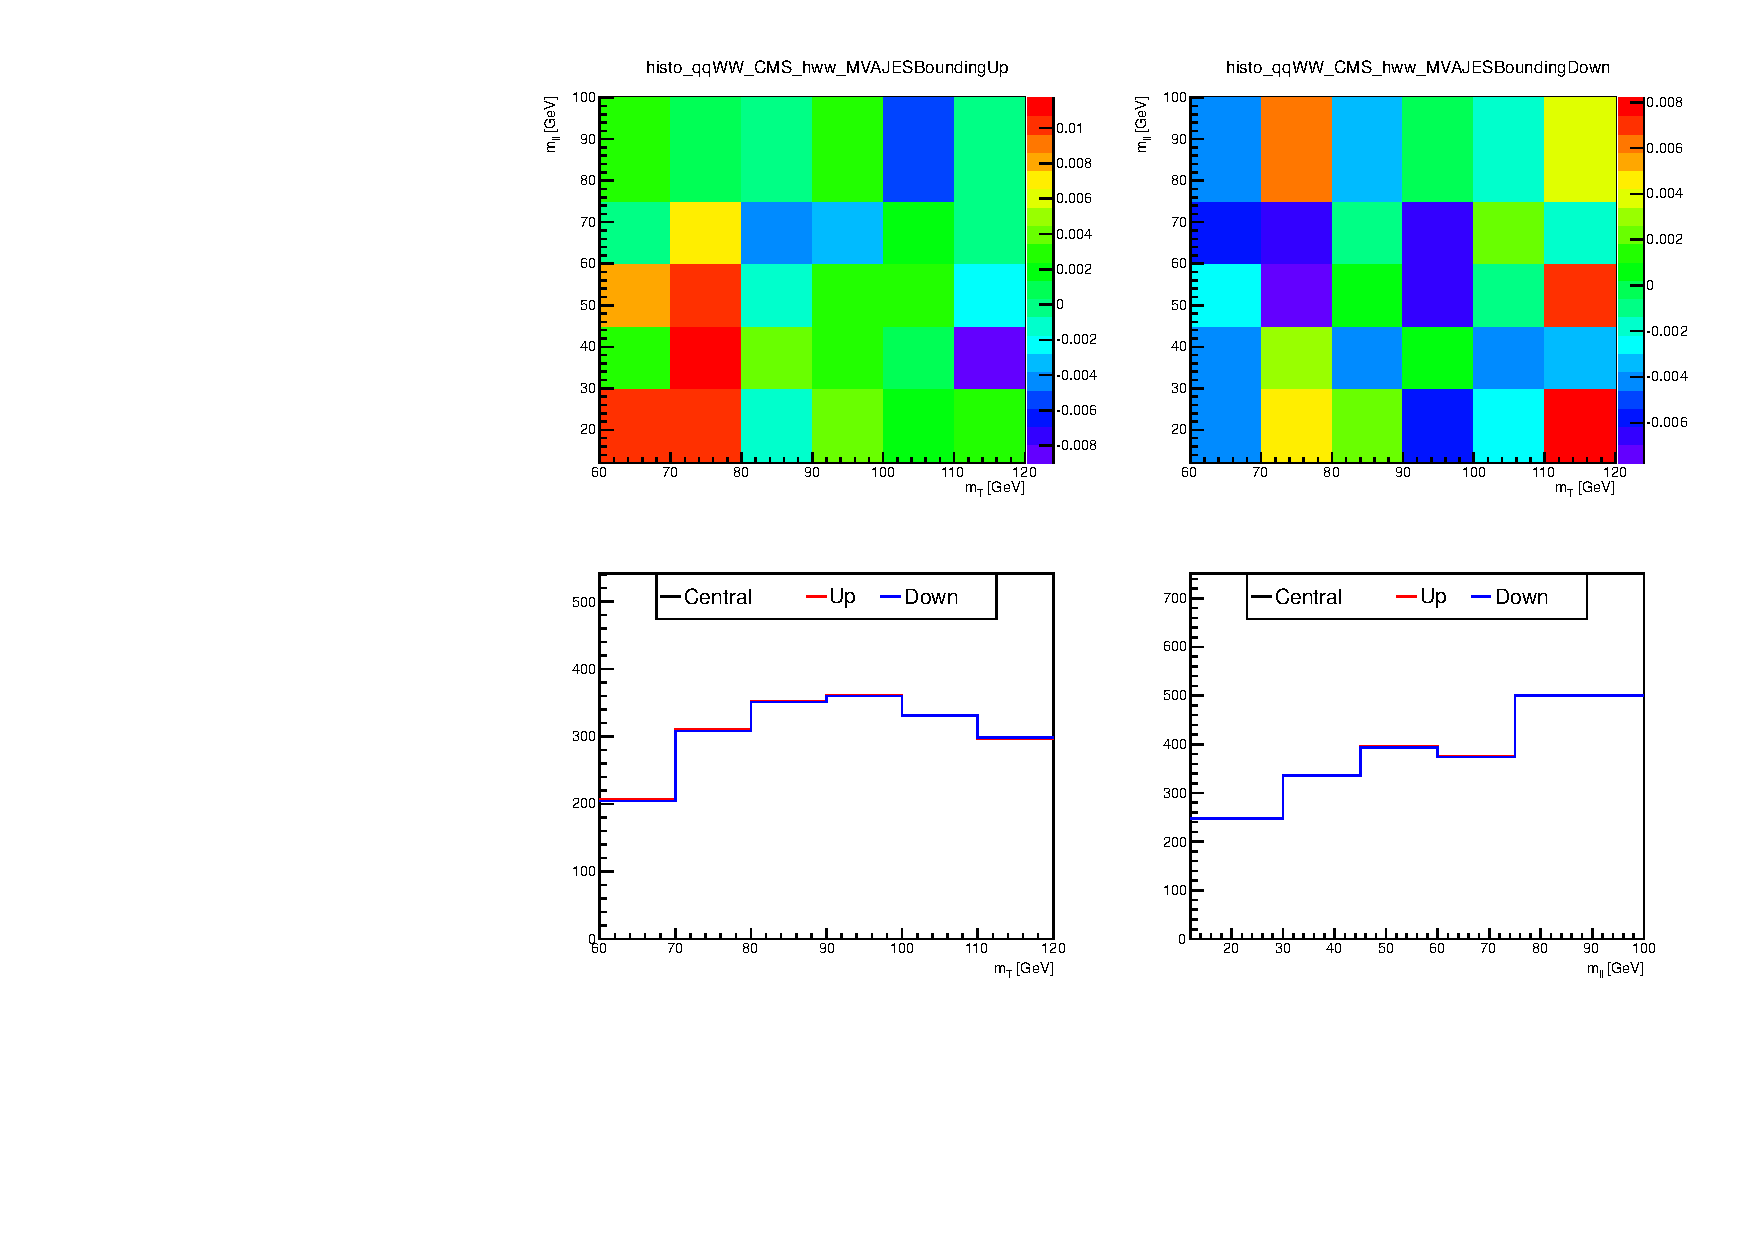
\includegraphics[width=0.8\textwidth]{figures/histo_qqWW_CMS_hww_MVAJESBounding_0j_zoom.pdf}
\end{tabular}
\caption{Alternate shapes for jet energy resolution.}
\label{fig:alter_jes}
\end{figure}

%%%
\subsubsection{MC statistics shape uncertainty} 

The limited statistics of the avaliable MC samples should be taken 
into account as a source of systematic uncertainty. 
For the cut-based analysis, overall statistical unceratianty of the sample 
after the final selection is taken into account. 
Fot the shape-based analysis, the up/down alternate shapes are constructed 
by adding/subtracting the size of statistical uncertainty in each bin. 
This does not allow bin-by-bin fluctuation in the statistical mechinary 
because all bins are either up or down by the statistical uncertainties 
in each bin. The ideal method should be considering each bin independently,
but this requires an extensive cpu time which is not in a realistic
time scale. We checked expected and observed significances of both methods 
and found that the results are compatible withn a few \%.  
Fig.~\ref{fig:alter_stat} shows the corresponding up/down alternate shapes
\ggww\ process in the 0-jet category. 
%
\begin{figure}[htp]
\centering
\begin{tabular}{c}
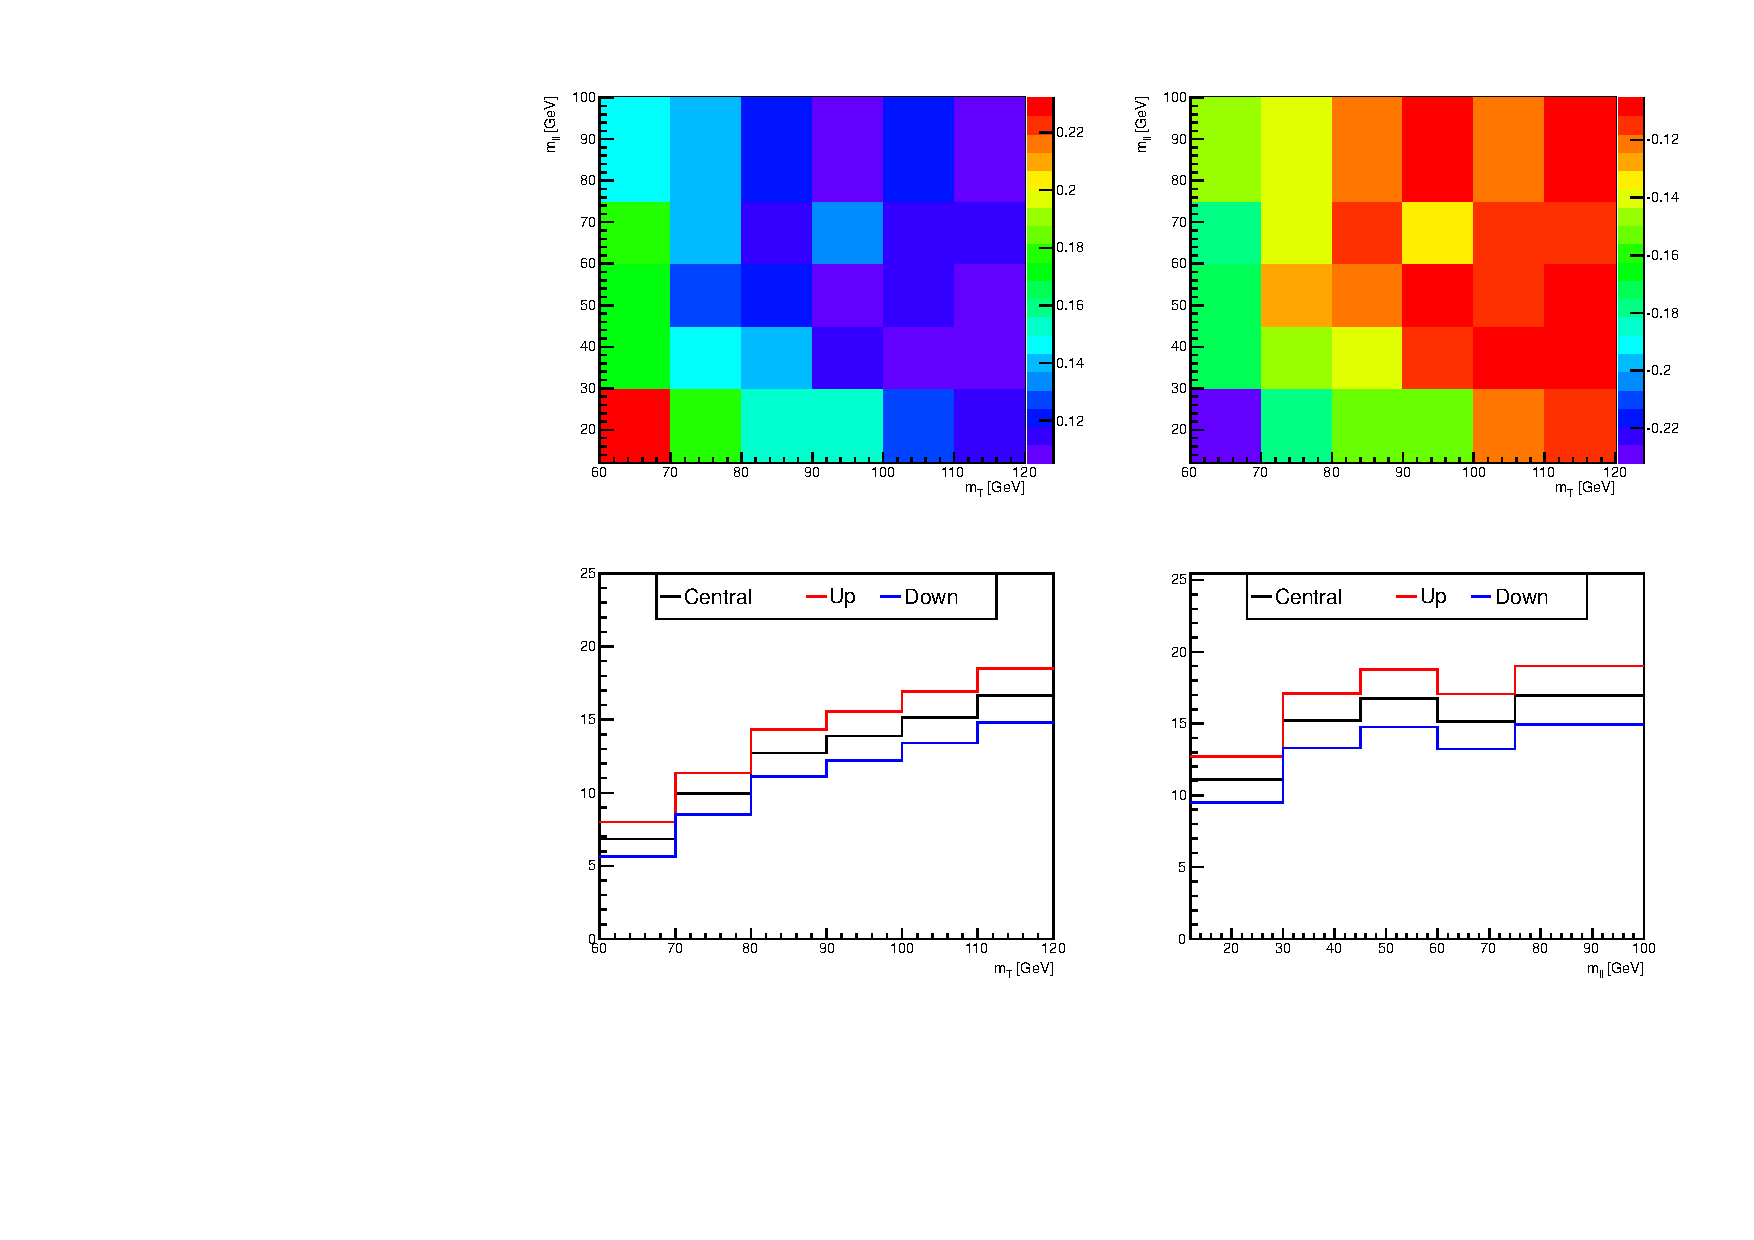
\includegraphics[width=0.8\textwidth]{figures/histo_ggWW_CMS_hww_of_0j_MVAggWWStatBounding_8TeV_0j_zoom.pdf}
\end{tabular}
\caption{Alternate shapes for MC statistics. \ggww }
\label{fig:alter_stat}
\end{figure}



%%%%%%%%%%%%%%%%%%%%%%%%%%%%%%%%%%%
\section{Background Estimation Uncertainty} 

The expected background contributions in the signal region are estimated by 
data-driven methods or taken from simulation after some data corrections.  
All procedures and the source of systematic uncertainties are discussed 
in chapter~\ref{ch:background_estimation}. These uncertainties are related 
to the normalizaion of each background. But, there is a shape systematics 
that can cause variation of shape. 

\subsubsection{\Wjets\ alternate shapes} 

As described in section~\ref{sec:wjets}, the \Wjets\ background is estimated 
by a data-driven method which measures the fake rate in QCD di-jet sample. 
One of the systematic sources is the variation of the away jet \pt
and the uncertainty of 30 \% is assigned to take this account. 
In the shape-based analysis, the affect of the varying the away jet \pt\ 
to the shape is considered as well. 
The alternate up shape is constructed using alternate jet \pt\ thresholds, 
15~\GeV for muons and 20~\GeV for electrons, and the relative difference 
in shape is taken. The alternate down shape is taken as a mirror of 
the up shape with respect to the central shape. 
Fig.~\ref{fig:alter_wjets} shows the corresponding up/down alternate shapes
for \Wjets\ when muon is an FO. 
%
\begin{figure}[htp]
\centering
\begin{tabular}{c}
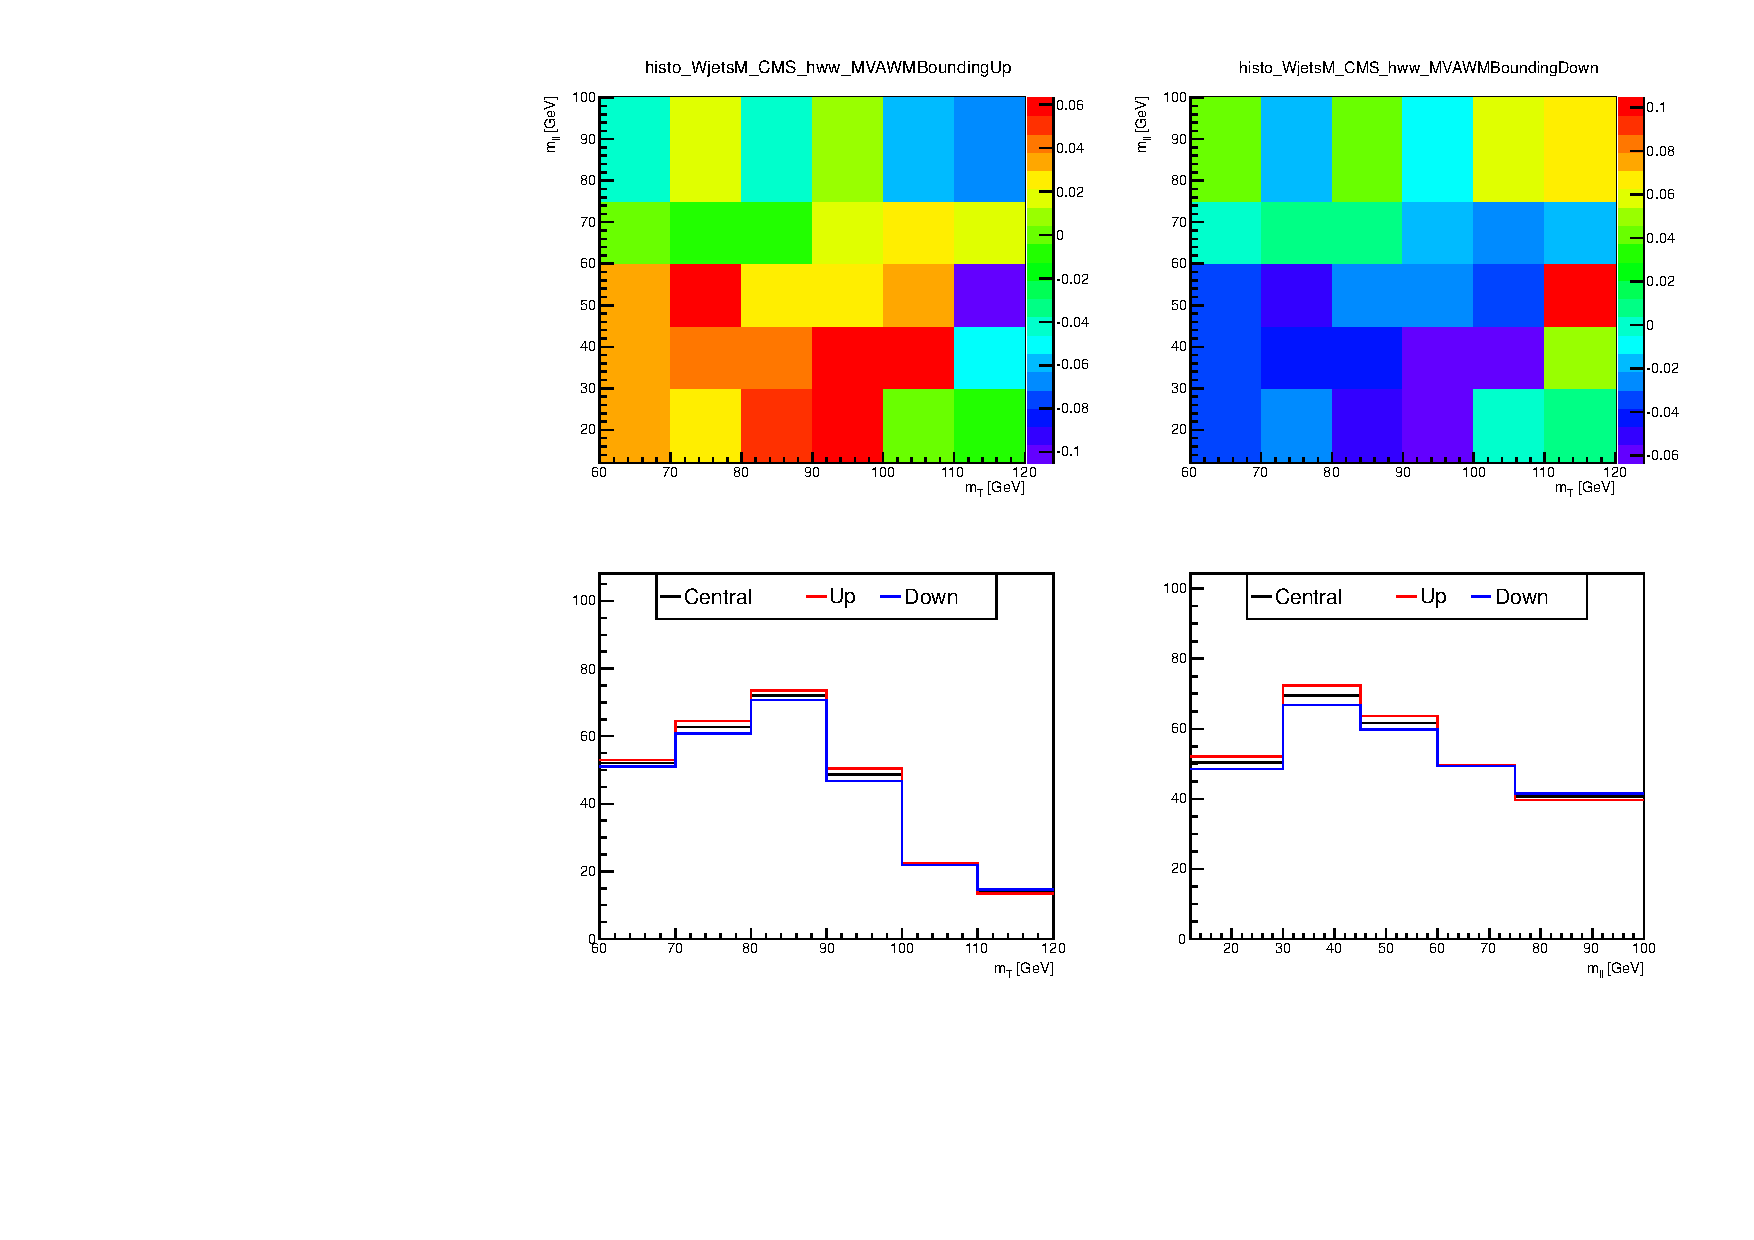
\includegraphics[width=0.8\textwidth]{figures/histo_WjetsM_CMS_hww_MVAWMBounding_0j_zoom.pdf}
\end{tabular}
\caption{Alternate shapes for \WjetsM. }
\label{fig:alter_wjets}
\end{figure}


%%%%%%%%%%%%%%%%%%%%%%%%%%%%%%%%%%% \section{Summary table?} 
